% \documentclass{beamer}
% \usetheme{Copenhagen}
% %\usecolortheme{beaver}

% \usepackage[utf8]{inputenc}


% \title{Oscillateur non-linéaires \& synchronisation}
% \author{Hervé Schmit-Veiler}
% \date{Septembre 2023}

% \begin{document}


% \maketitle

% \begin{frame}{Introduction}

    

% \end{frame}

% \begin{frame}{Résonance harmonique}

% \end{frame}

% \begin{frame}{Oscillateur de Duffing - 1}
    
% \end{frame}

% \begin{frame}{Moyennement}
    
% \end{frame}



% \end{document}

\documentclass{beamer}

\usetheme{Madrid}
%\usecolortheme{seagull}
\usepackage[utf8]{inputenc}
\usepackage{graphicx}
\usepackage{amsmath}
\usepackage{breqn} % for dmath env

\usepackage[
            backend=biber,
            style=numeric,
            %langid=french,
            sorting=none,
            ]{biblatex}
\DeclareNameAlias{author}{last-first}

\addbibresource{refs/ref_v11.bib}

% Title slide
\title{Oscillations non-linéaires et syncrhonisation}
\author{Hervé Schmit-Veiler}
%\institute{Université de Bordeaux}
\date{\today}

\begin{document}

\frame{\titlepage}

\small

% Outline slide
\begin{frame}{Plan}
  \tableofcontents
\end{frame}



% Section 1: Introduction
\section{Introduction}
\begin{frame}{Introduction}
  \begin{itemize}
    \item Stage au LOMA
    \item Étude de systèmes d'oscillateurs non-linéaires
    \item But : appliquer ces méthodes d'analyse à un système d'oscillateurs non-linéaires couplées
    \item Applications
    \begin{itemize}
      \item Radios, lasers
      \item Qubits \cite{pistolesi_proposal_2021}, detecteurs de force ultrasensible \cite{moser_ultrasensitive_2013}
    \end{itemize}
  \end{itemize}
\end{frame}

% Section 2: Non-Linear Oscillator Models
\section{Oscillateur Harmonique}
\begin{frame}{Oscillateur Harmonique Forcé}

    %\begin{minipage}{0.5\textwidth}
    $$ \ddot{x} + \gamma\dot{x} + \omega_0^2 x = \frac{F_0}{m}\cos(\omega t) $$

    \begin{itemize}
        \item Réponse fréquentielle lorenztienne
        \item Régime permanent qui ne dépend que des paramètres de l'équation
    \end{itemize}
    
    %\end{minipage}

    %\begin{minipage}{0.45\textwidth}
        \begin{figure}
            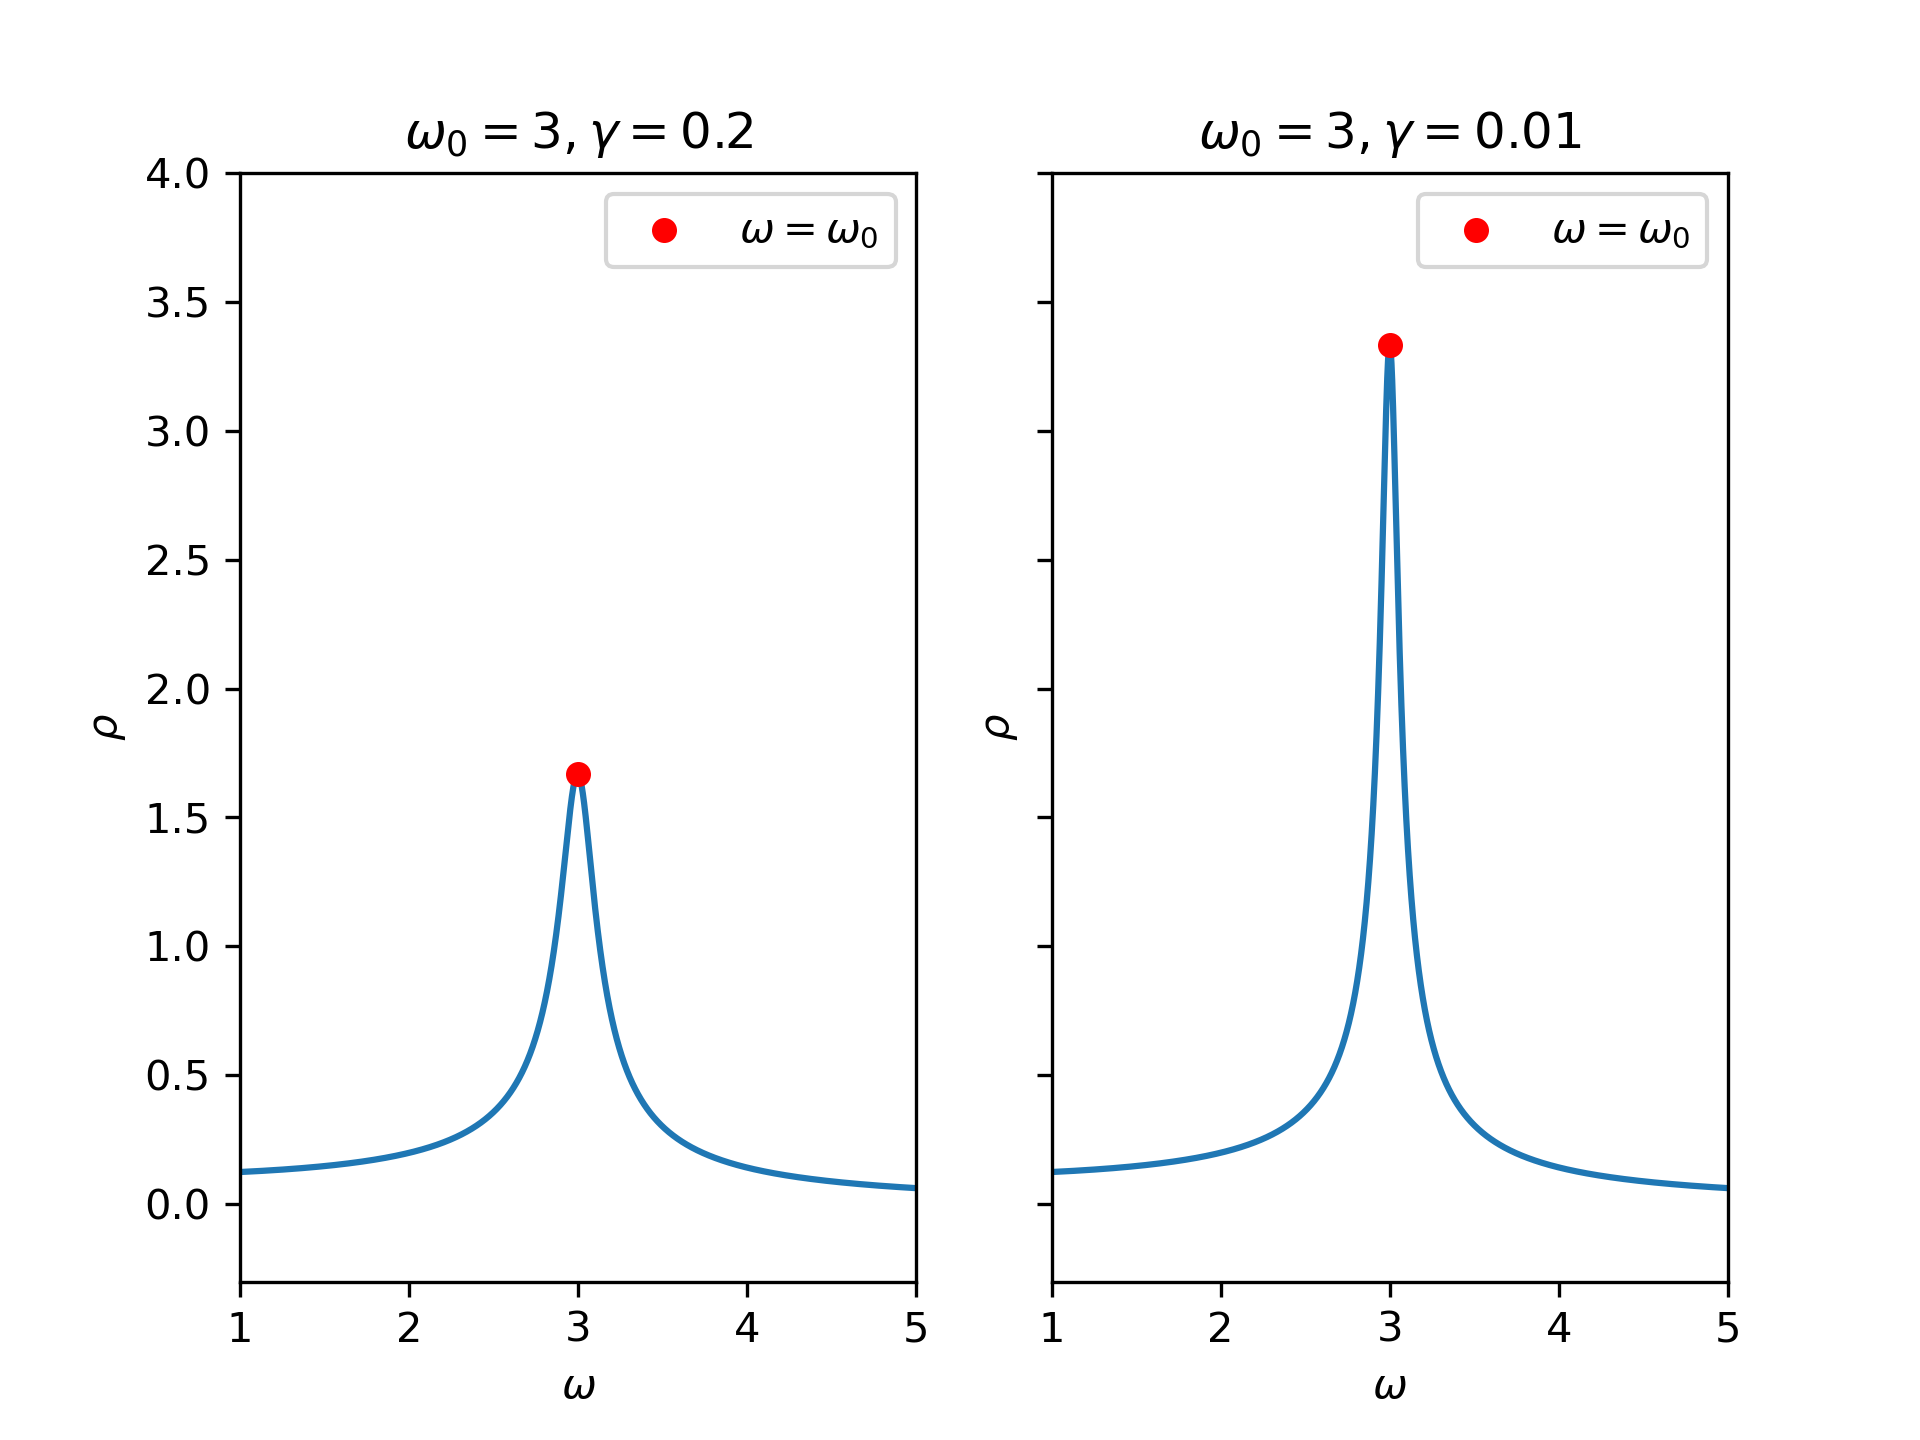
\includegraphics[width=0.45\textwidth]{images/harmonique/rho_plot_contrast.png}
            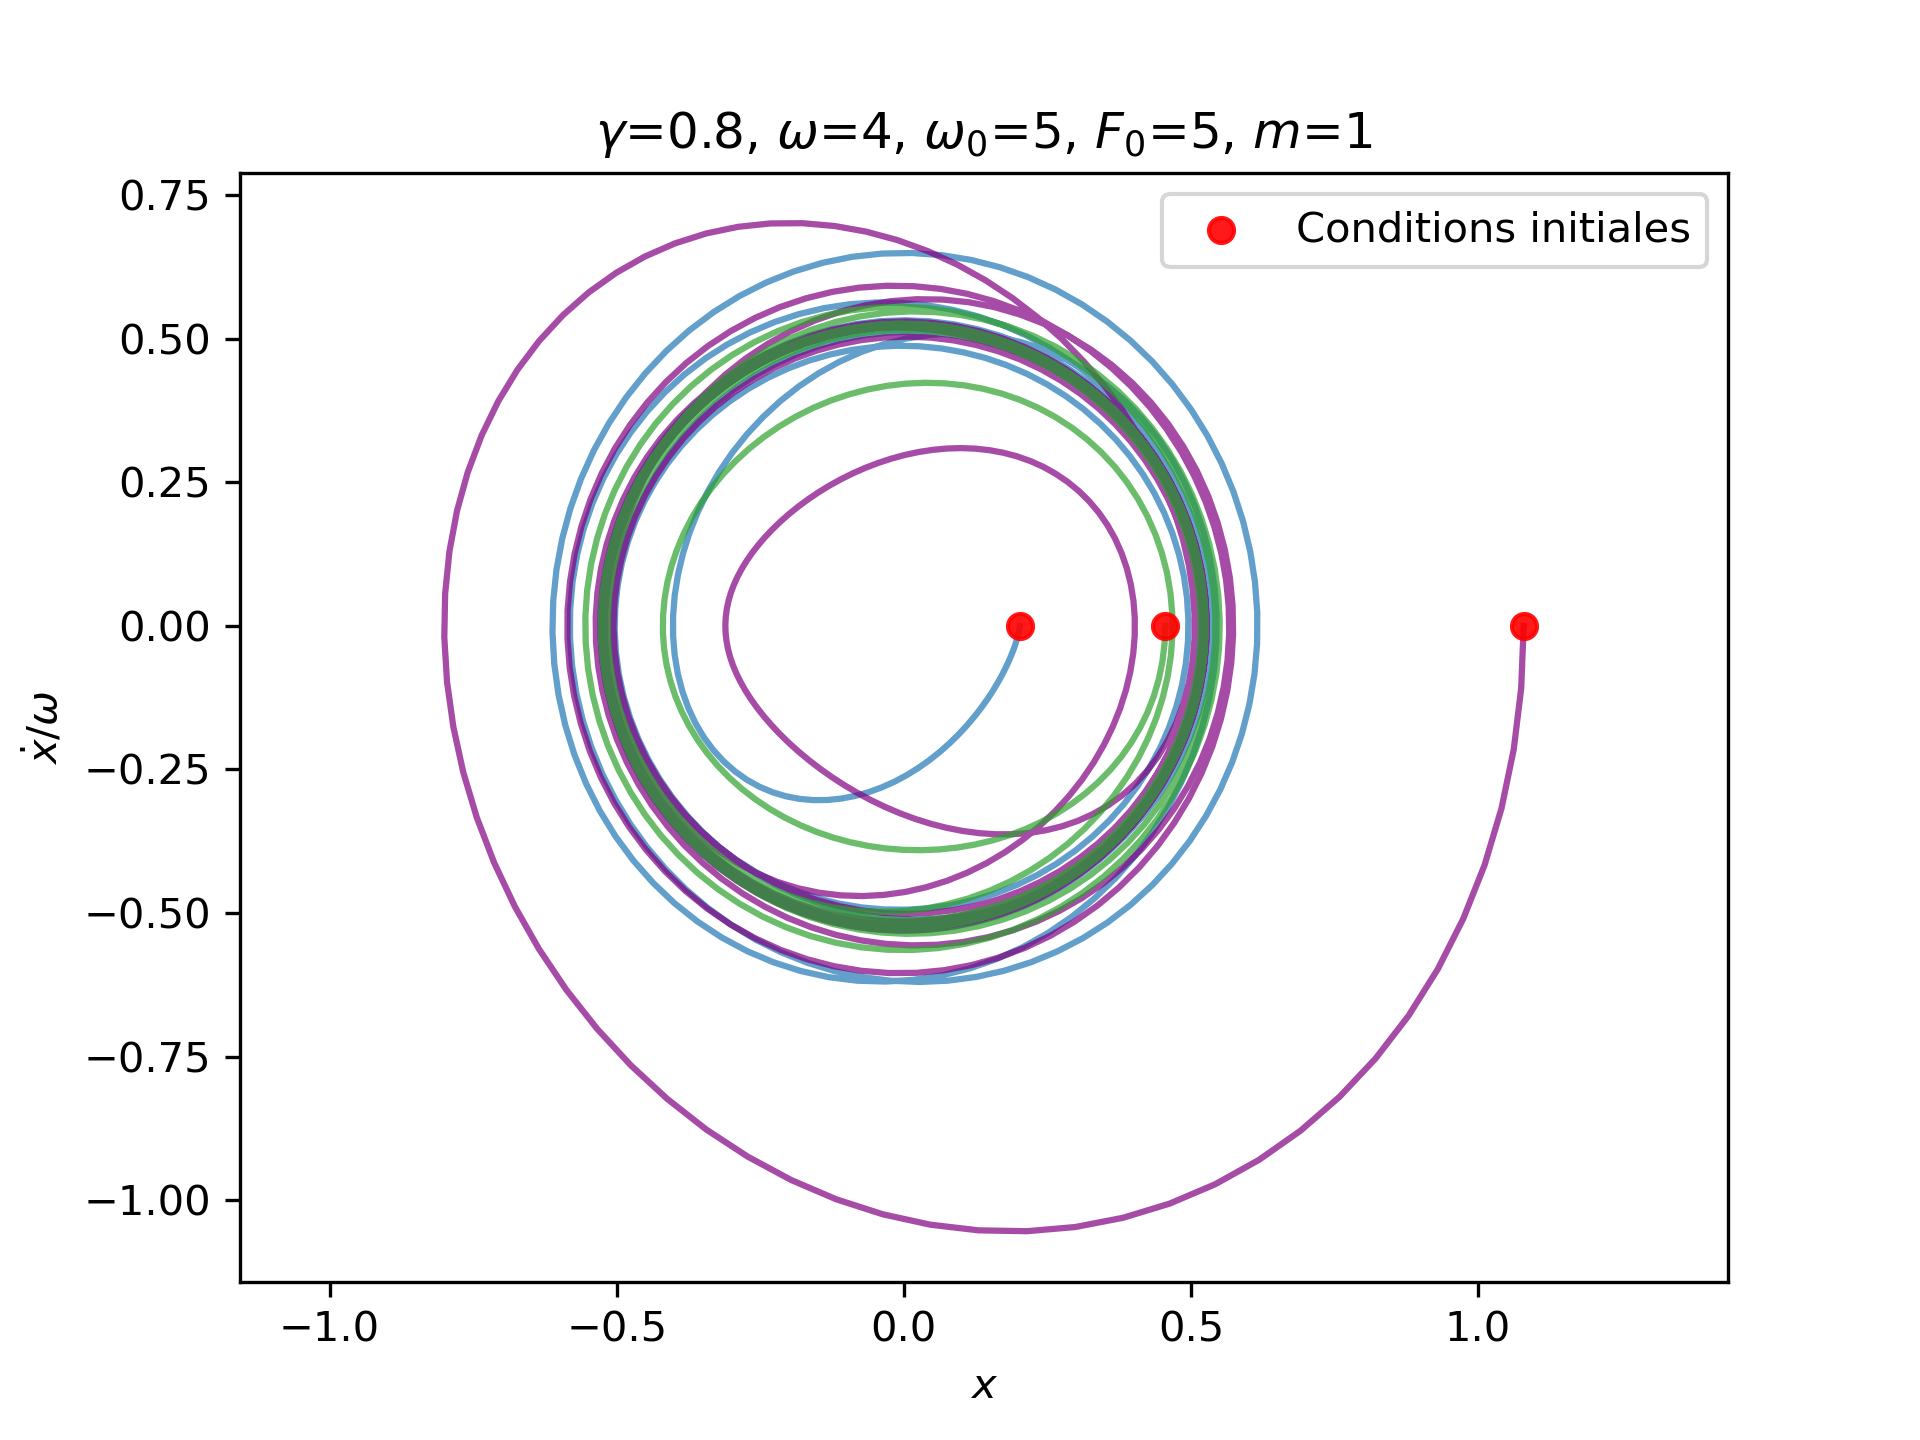
\includegraphics[width=0.45\textwidth]{images/harmonique/ho_triple_phase_plot_x0=0.532808128684573_v0=0_gamma=0.8_w0=5_w=4_f0=5.png}
        \end{figure}
    %\end{minipage}
    
    %\begin{itemize}
    %    \item $ \ddot{x} + \gamma\dot{x} + \omega_0^2 x = \frac{F_0}{m}\cos(\omega t) $
    %    \item 
    %  \end{itemize}
      % add phase plot, and plot of frequency response and phase
\end{frame}

\section{Oscillateurs non-linéaires}
\begin{frame}{Oscillateur de Duffing - 1}
    $$ \ddot{x} + \omega_0^2 x + \gamma \dot{x} + \alpha x^3 = f_0\cos(\omega t)$$
    
    \begin{itemize}
        \item Modèle pour structures elastiques en régime forcé et pour grandes amplitudes \cite{rand_lecture_2012}
        \item Régime permanent presque harmonique pour des 'petits' paramètres
        \item Doublement des periodes si $f_0$ augmente suffisament (chaos)
    \end{itemize}

    \begin{figure}
        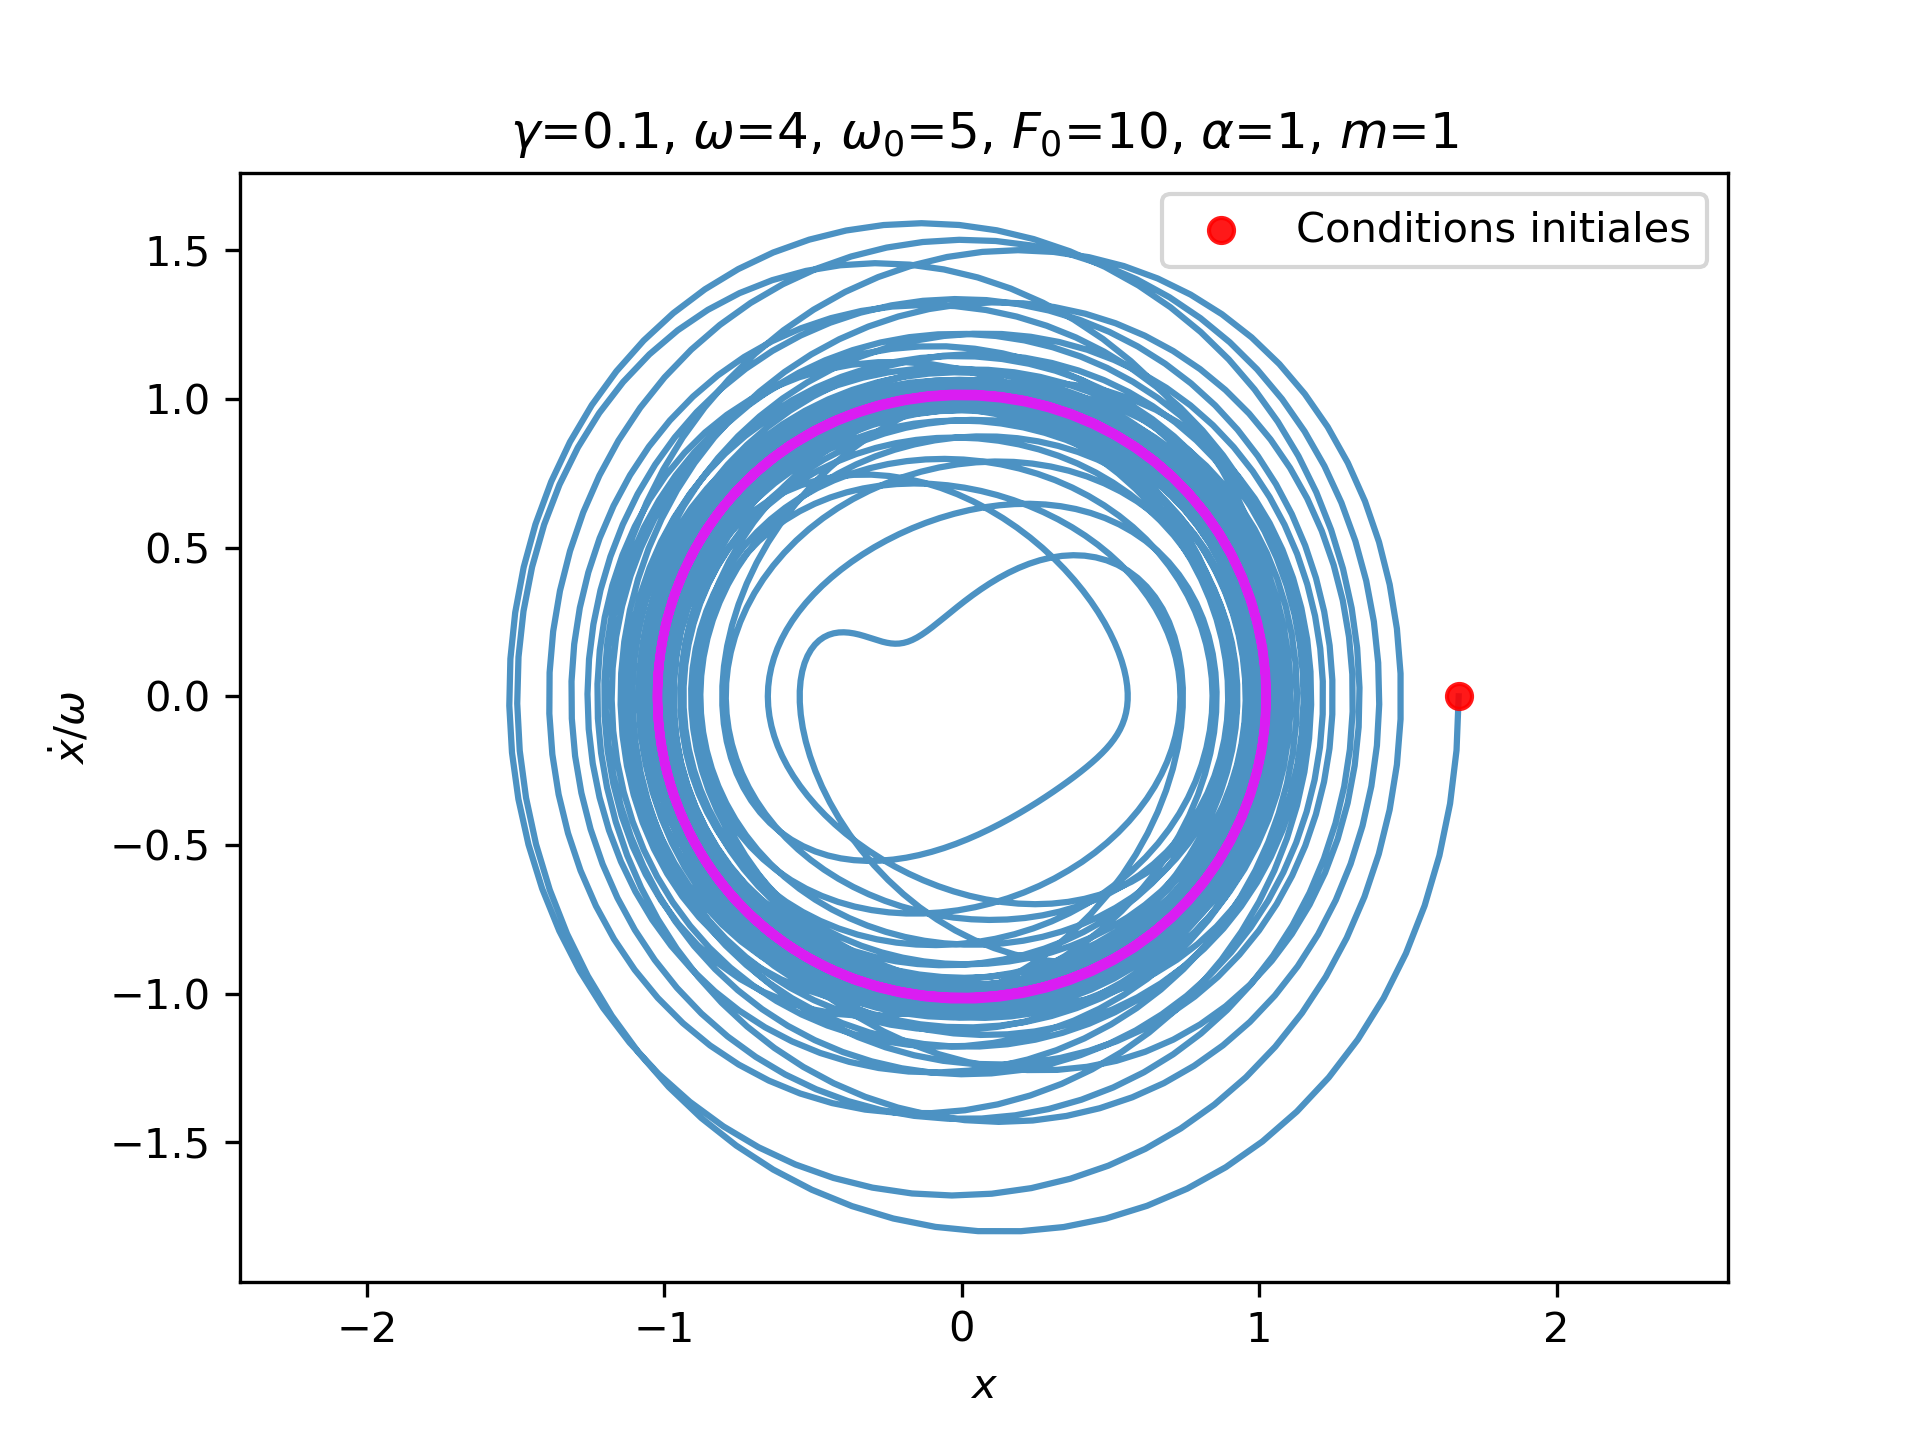
\includegraphics[width=0.32\textwidth]{images/duffing/duffing_single_phase_plot_x0=0.4750630195324652_v0=0_gamma=0.1_w0=5_w=4_f0=10_alpha=1_epsilon=1.png}
        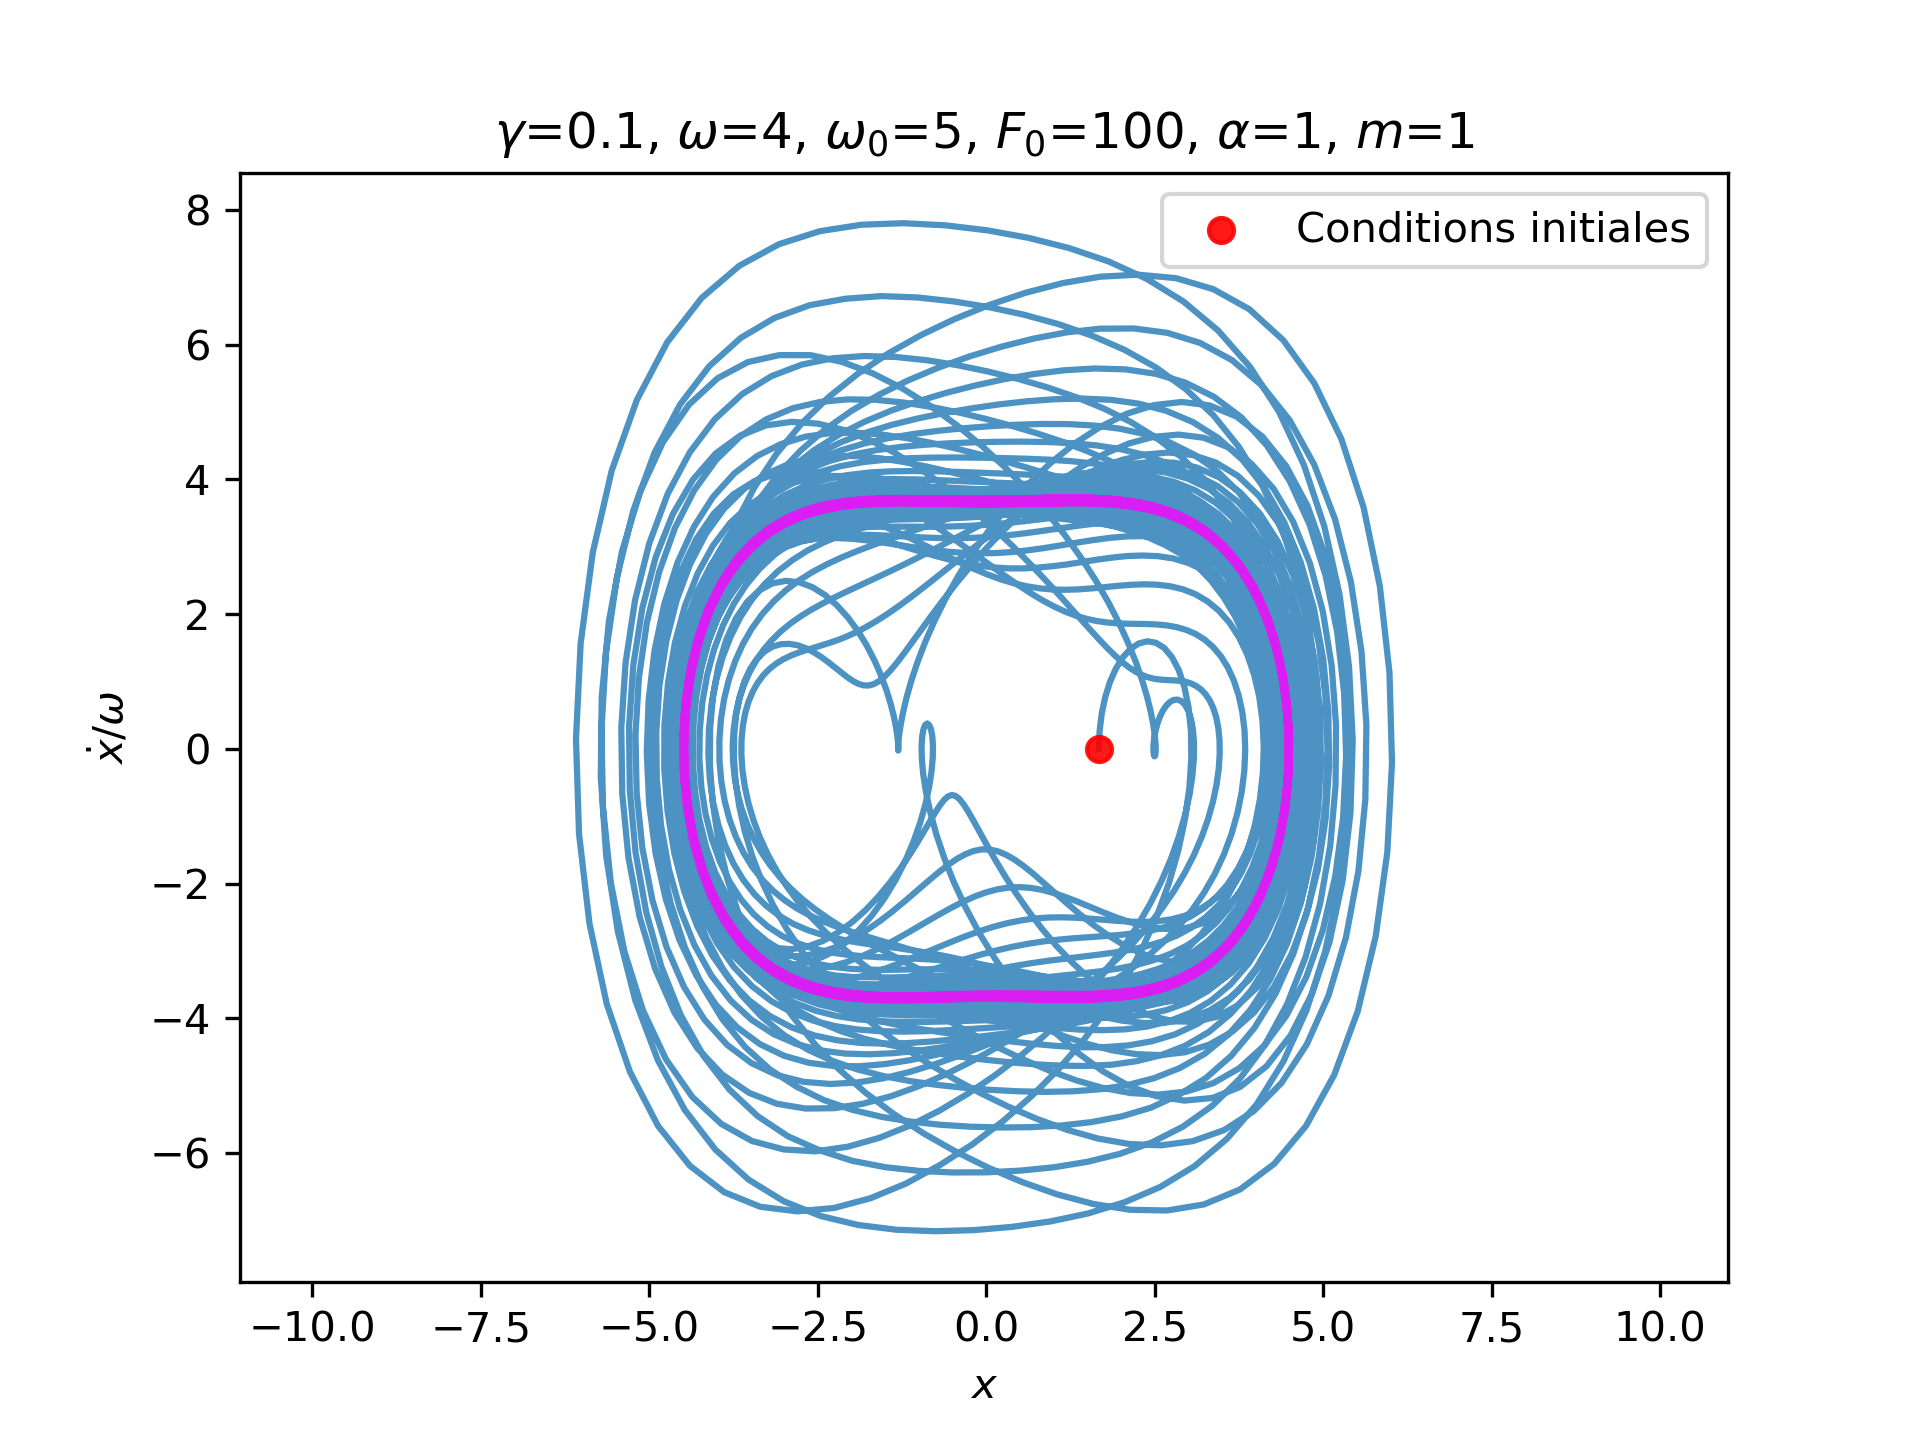
\includegraphics[width=0.32\textwidth]{images/duffing/duffing_single_phase_plot_x0=0.4750630195324652_v0=0_gamma=0.1_w0=5_w=4_f0=100_alpha=1_epsilon=1.png}
        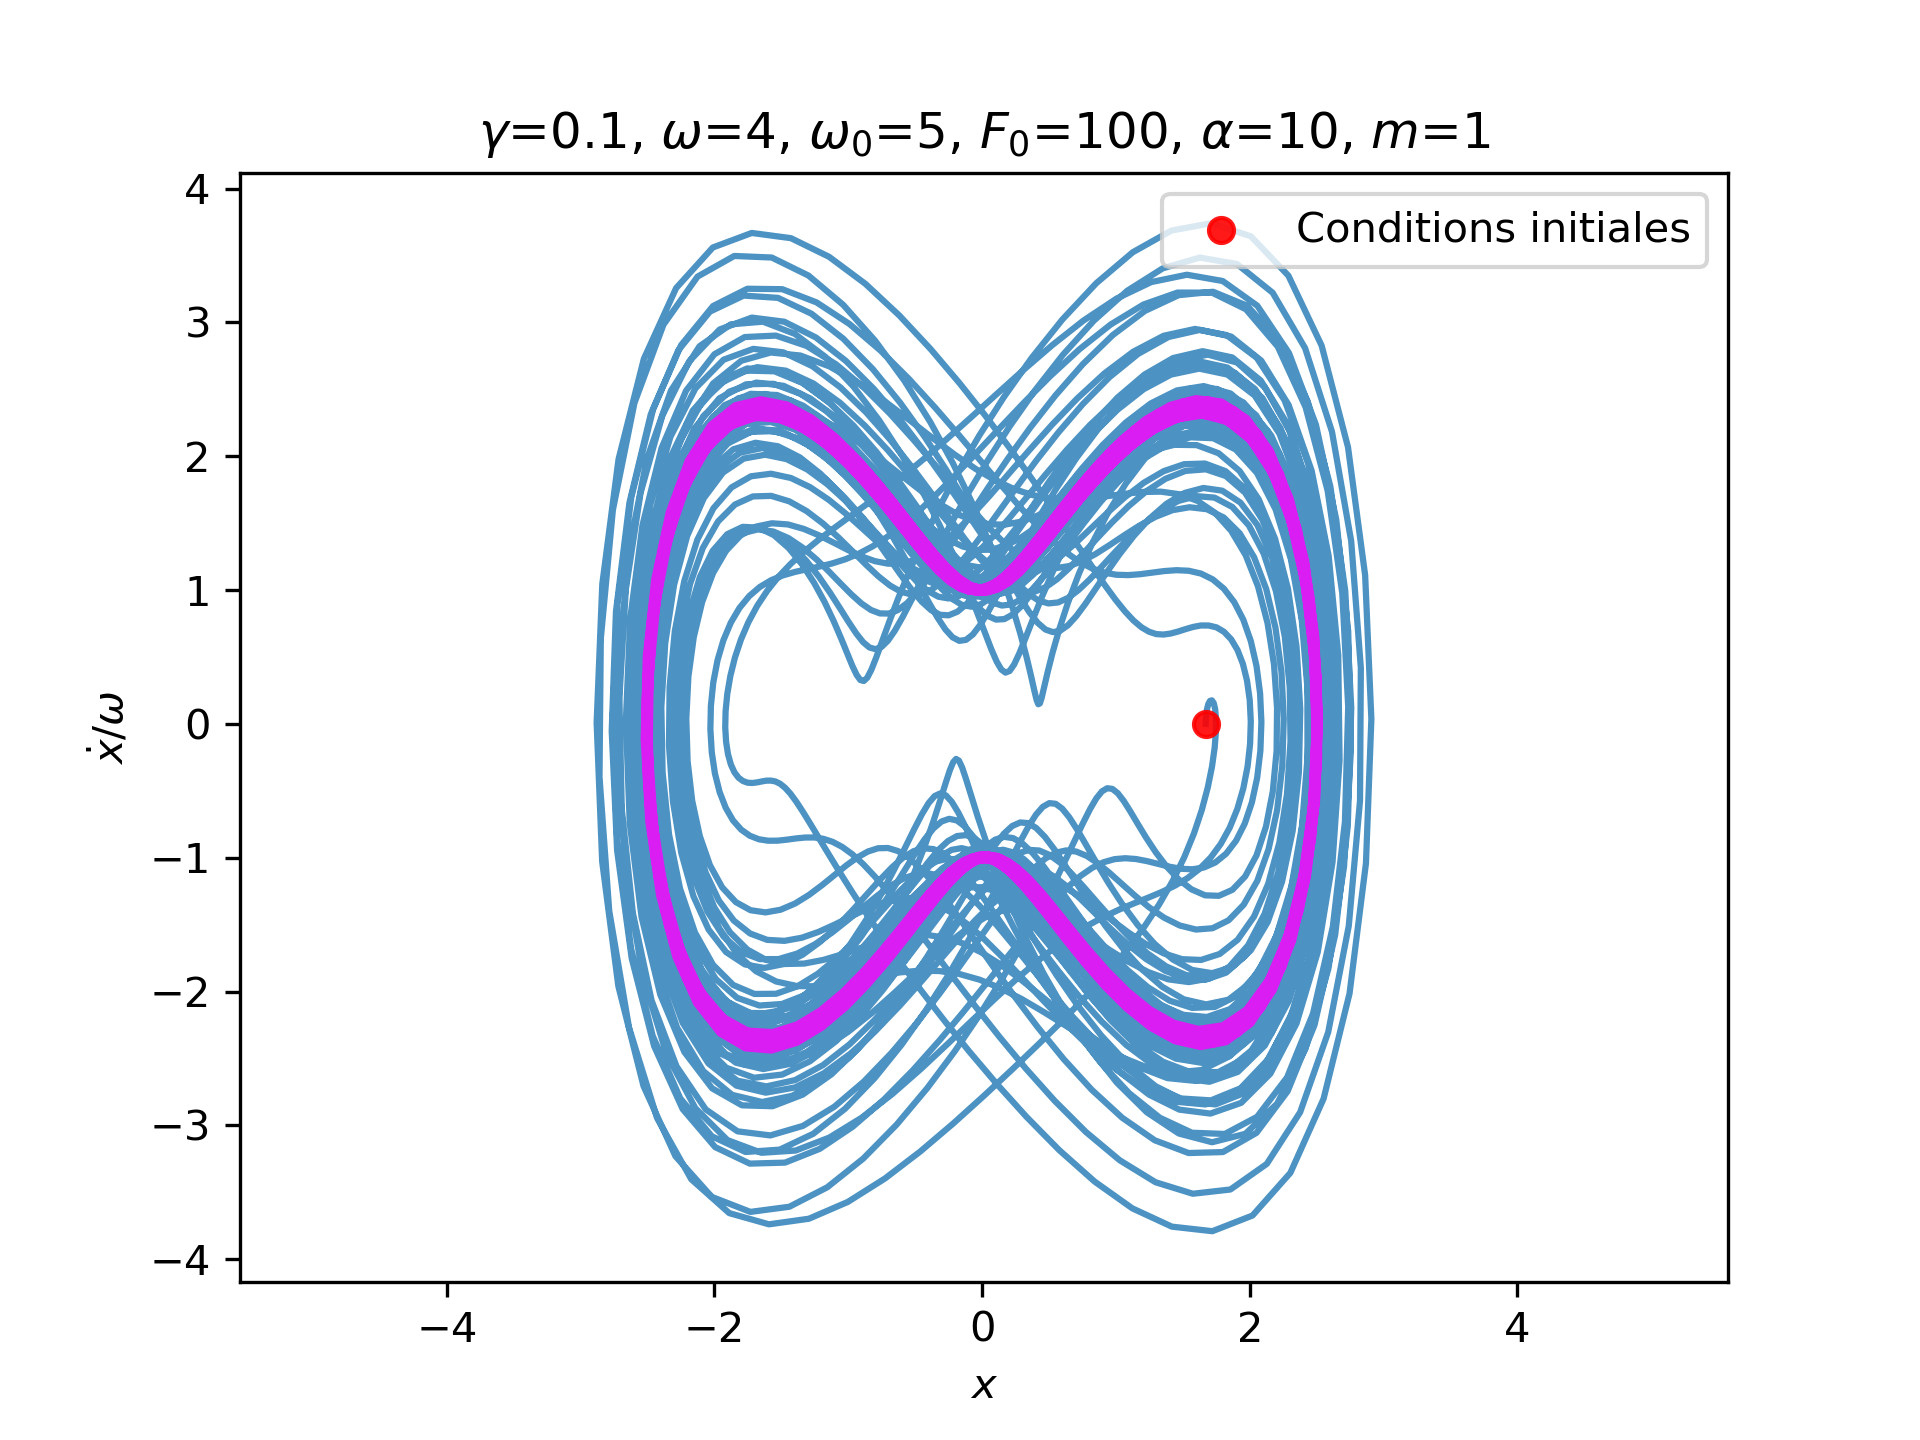
\includegraphics[width=0.32\textwidth]{images/duffing/duffing_single_phase_plot_x0=0.4750630195324652_v0=0_gamma=0.1_w0=5_w=4_f0=100_alpha=10_epsilon=1.png}
    \end{figure}

    \begin{center}{\tiny Régime permanent en magenta}\end{center}
\end{frame}

\begin{frame}{Moyennement}
    $$ \ddot{x} + \omega_0^2 x = \epsilon f(\dot{x}, x, t) \qquad 0 < \epsilon \ll \omega_0 $$
    \begin{itemize}
        \item Méthodes d'analyse approximative pour équations harmoniques perturbés
        \item On suppose pouvoir trouver solutions sous la forme \cite{rand_lecture_2012} :
            $$x(t) = r(t)\cos(\omega_0 t + \phi(t)) \qquad \dot{x}(t) =  -\omega_0 r(t)\sin(\omega_0 t + \phi(t))$$
        %\item Remarque : on ne considère pas les contributions de $\dot{r}$ et de $\dot{\phi}$
        \item $r(t)$ et $\phi(t)$ sont lentement variable pour petit $\epsilon$, permet de faire moyennement au premier ordre
            $$ r(t) \approx \langle r \rangle \qquad \phi(t) \approx \langle \phi \rangle $$
    \end{itemize}
\end{frame}

\begin{frame}{Oscillateur de Duffing - 2}
  %\begin{itemize}
  \begin{equation*}
    x(t) = z(t)e^{i\omega t} + \bar{z}(t) e^{-i\omega t}
    \qquad 
    \dot{x}(t) = i\omega \left[ z(t)e^{i\omega t} - \bar{z}(t) e^{-i\omega t} \right]
    \label{eq:duff_x_xdot_exp}
  \end{equation*}
  \begin{itemize}
    \item Substitution dans l'équation différentielle
  \end{itemize}
  \begin{dmath*}
    2i\omega \dot{z}(t)e^{i\omega t} + (i\omega)^2 \left[ z(t)e^{i\omega t} + \bar{z}(t) e^{-i\omega t} \right]
    + i\epsilon\gamma\omega \left[ z(t)e^{i\omega t} - \bar{z}(t) e^{-i\omega t} \right] \\
    + \omega_0^2 \left[ z(t)e^{i\omega t} + \bar{z}(t) e^{-i\omega t} \right]
    + \epsilon \alpha \left[ z(t)e^{i\omega t} + \bar{z}(t) e^{-i\omega t} \right]^3 = \epsilon \frac{f_0}{2}\left[ e^{i\omega t} + e^{-i\omega t} \right]
  \end{dmath*}
  \begin{itemize}
    \item Moyennement
  \end{itemize}
  \begin{dmath*}
    2i\omega \dot{z}
    = (\omega^2 - \omega_0^2)z(t) - i\epsilon\gamma\omega z(t) - 3\epsilon\alpha |z|^2 z(t) + \epsilon \frac{f_0}{2}
  \end{dmath*}
  \begin{itemize}
    \item Adimensionnement
  \end{itemize}
  \begin{equation*}
    q'(\tau) = -i\Omega q(\tau) - q(\tau) + i|q|^2q(\tau) - F_0
  \end{equation*}
  %\tiny
  \begin{equation*}
    \tau = \frac{\epsilon\gamma}{2}t
    \qquad
    q(\tau) = \sqrt{\frac{3\alpha}{\omega\gamma}}z(t)
    \qquad
    \Omega = \frac{(\omega - \omega_0)}{\epsilon\gamma/2}
    \qquad
    F_0 = \frac{\sqrt{3\alpha}f_0}{2(\omega \gamma)^{3/2}}
  \end{equation*}
  \small
 
\end{frame}

\begin{frame}{Oscillateur de Duffing - 3}
  \begin{itemize}
    \item Après moyennement et adimensionnement, on trouve l'amplitude complexe $q_0$ du régime permanent pour $\omega \approx \omega_0$ \cite{pistolesi_duffing_nodate}. $\Omega \propto (\omega-\omega_0)$
        $$  q_0 = \frac{F_0}{|q_0|^2 - \Omega + i} \implies \Omega = |q_0|^2 \pm \sqrt{\frac{F_0^2}{|q_0|^2} - 1 } $$
    \item Bistabilité d'amplitude et hystérèse \cite{landau_mechanics_1976}
  \end{itemize}
    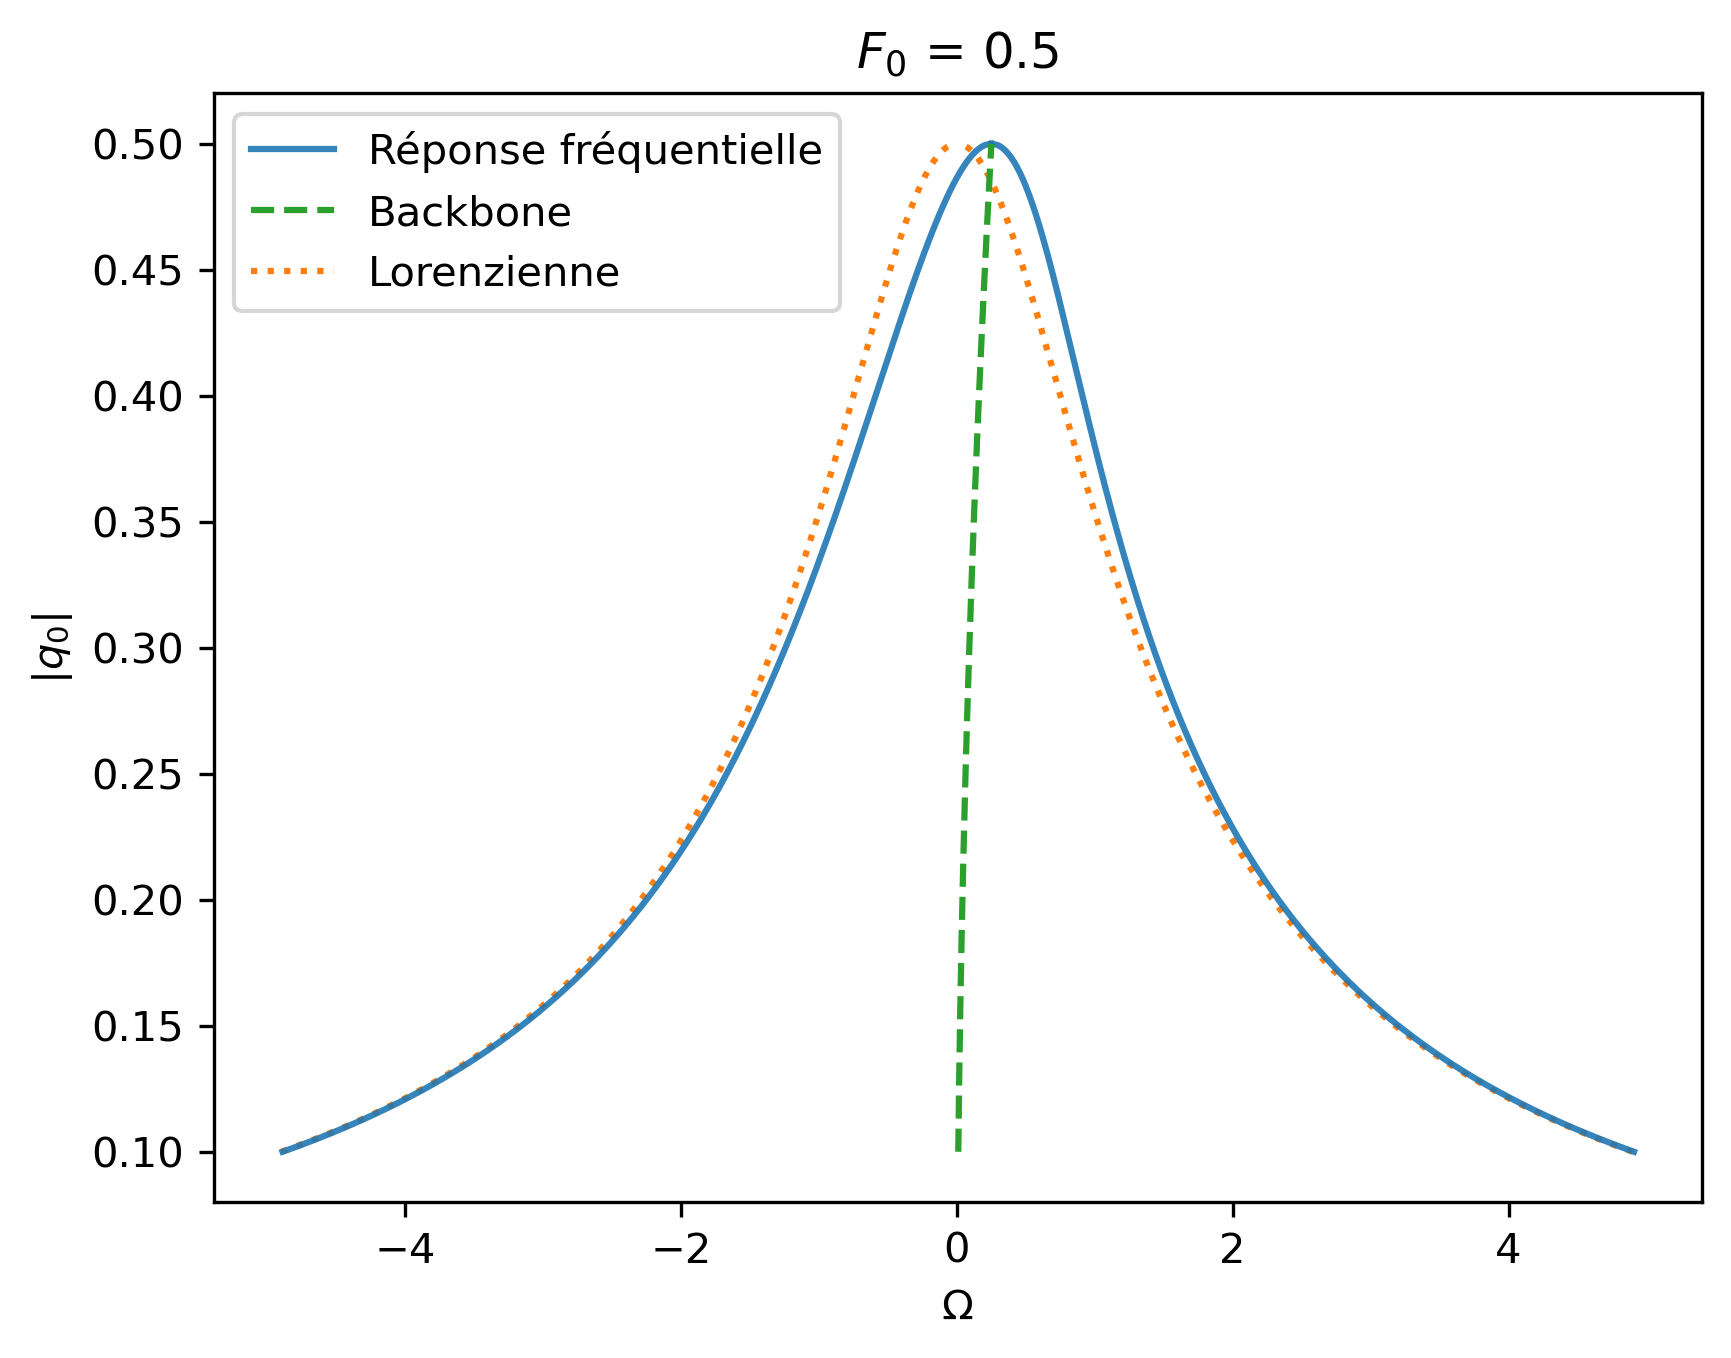
\includegraphics[width=0.32\textwidth]{images/duffing/F0=0.5.png}
    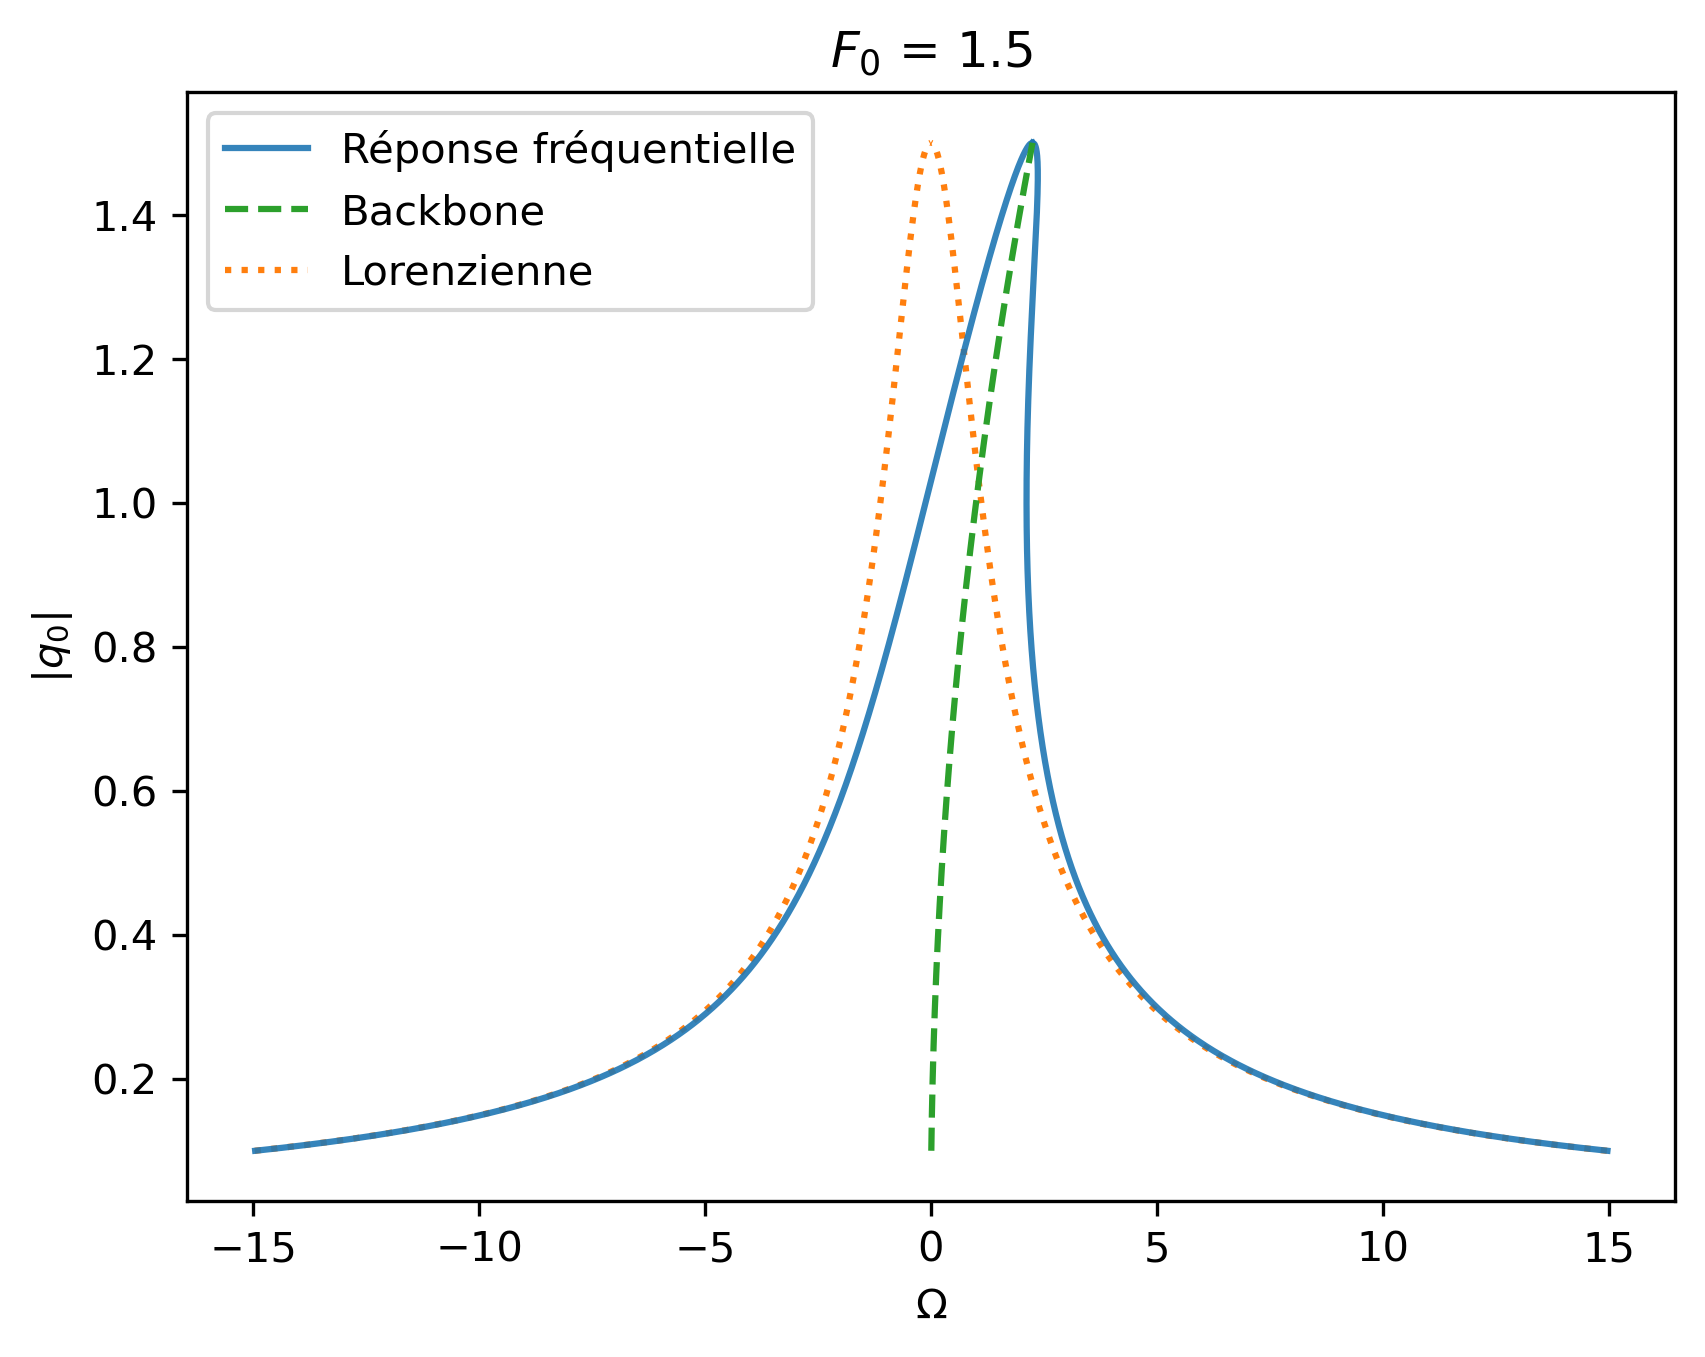
\includegraphics[width=0.32\textwidth]{images/duffing/F0=1.5.png}
    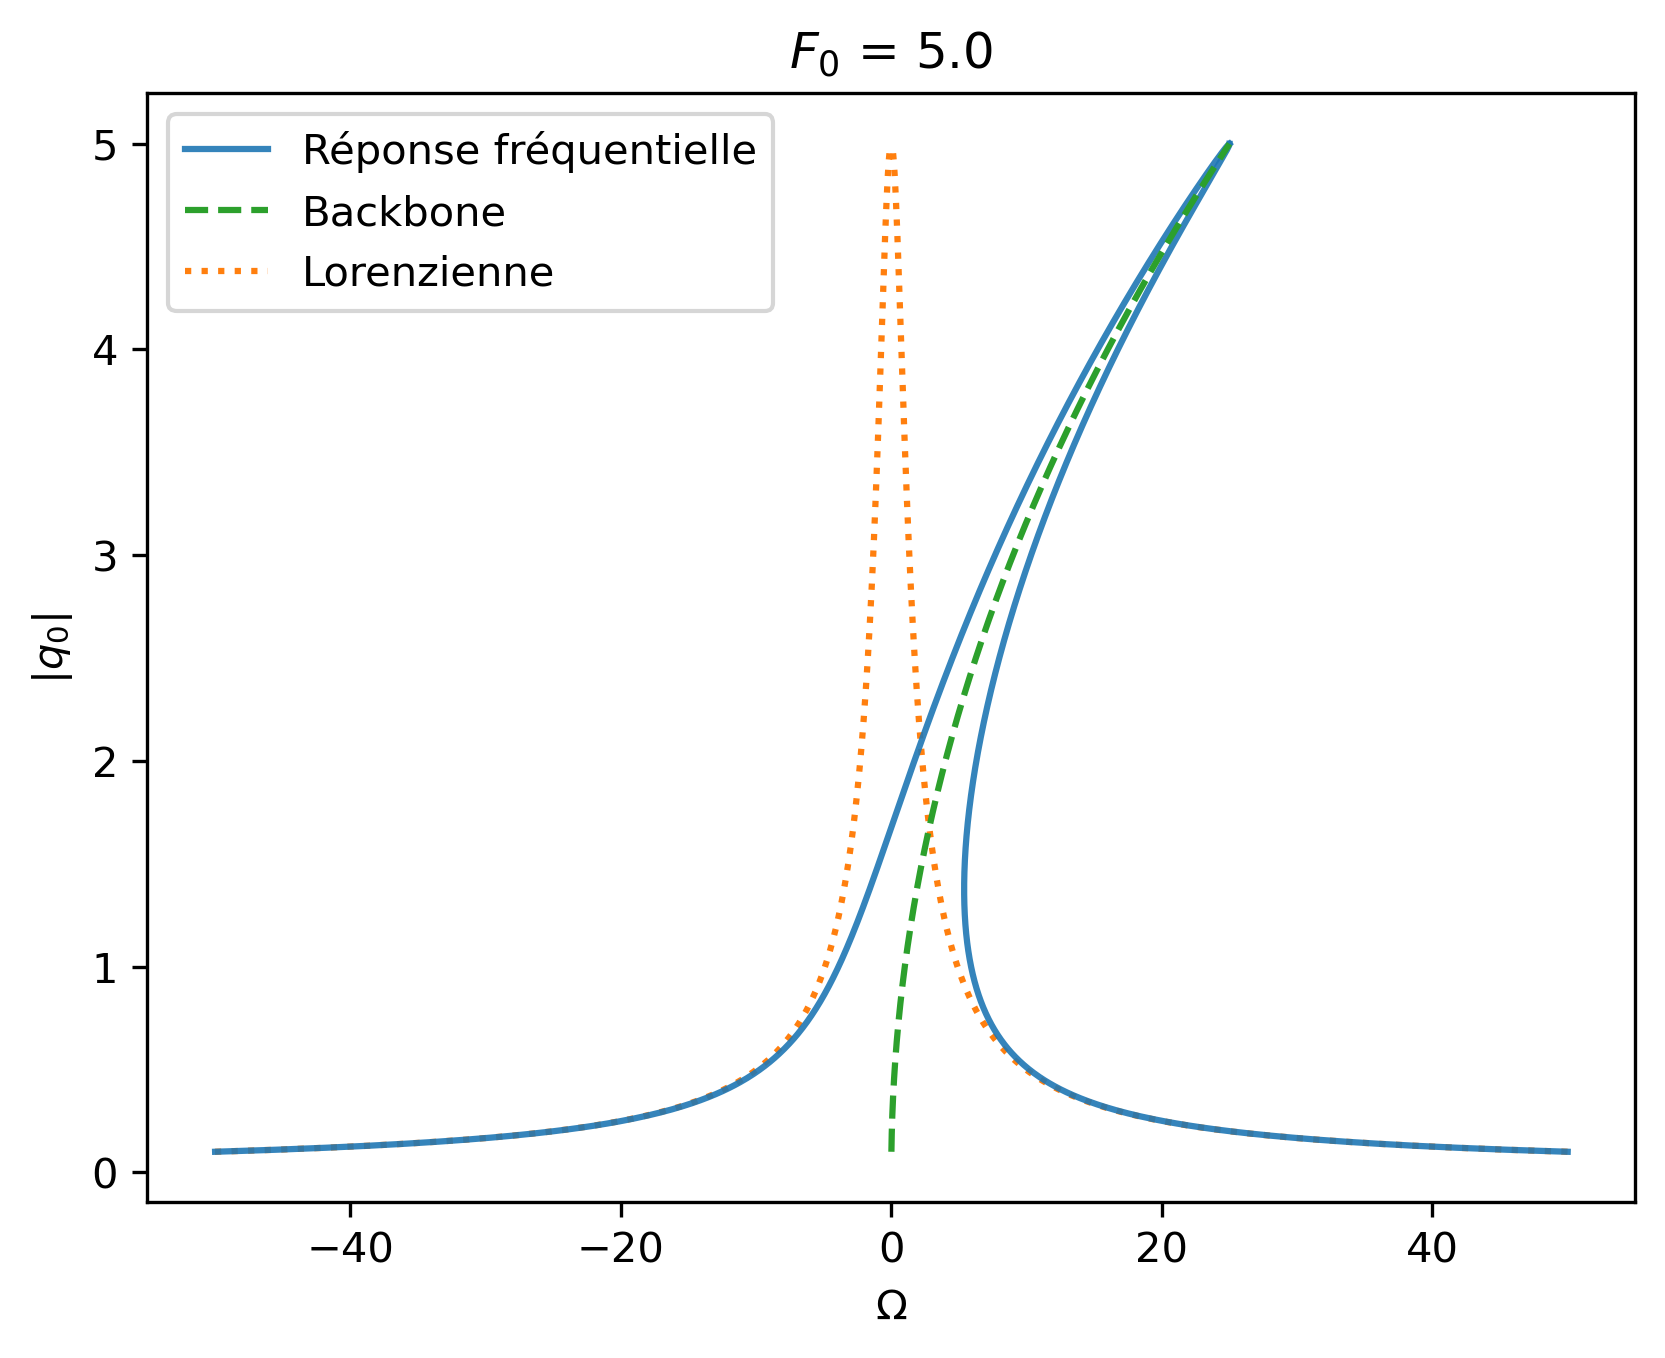
\includegraphics[width=0.32\textwidth]{images/duffing/F0=5.0.png}
\end{frame}

%\section{Oscillateur de Van der Pol}
\begin{frame}{Oscillateur de Van der Pol - 1}
    $$ \ddot{x}  +  x + \epsilon(x^2 - 1)\dot{x} = 0 $$
    \begin{itemize}
        \item Modèle simple d'un oscillateur présentant un cycle limite
        \begin{itemize}
            \item unique orbite isolée dans l'espace de phase
        \end{itemize}
        \item Signe changeant du terme en $\dot{x}$ qui injecte/dissipe de l'énergie
        \item Cycle limite quasi-circulaire pour petit $\epsilon$
    \end{itemize}

    \begin{figure}
        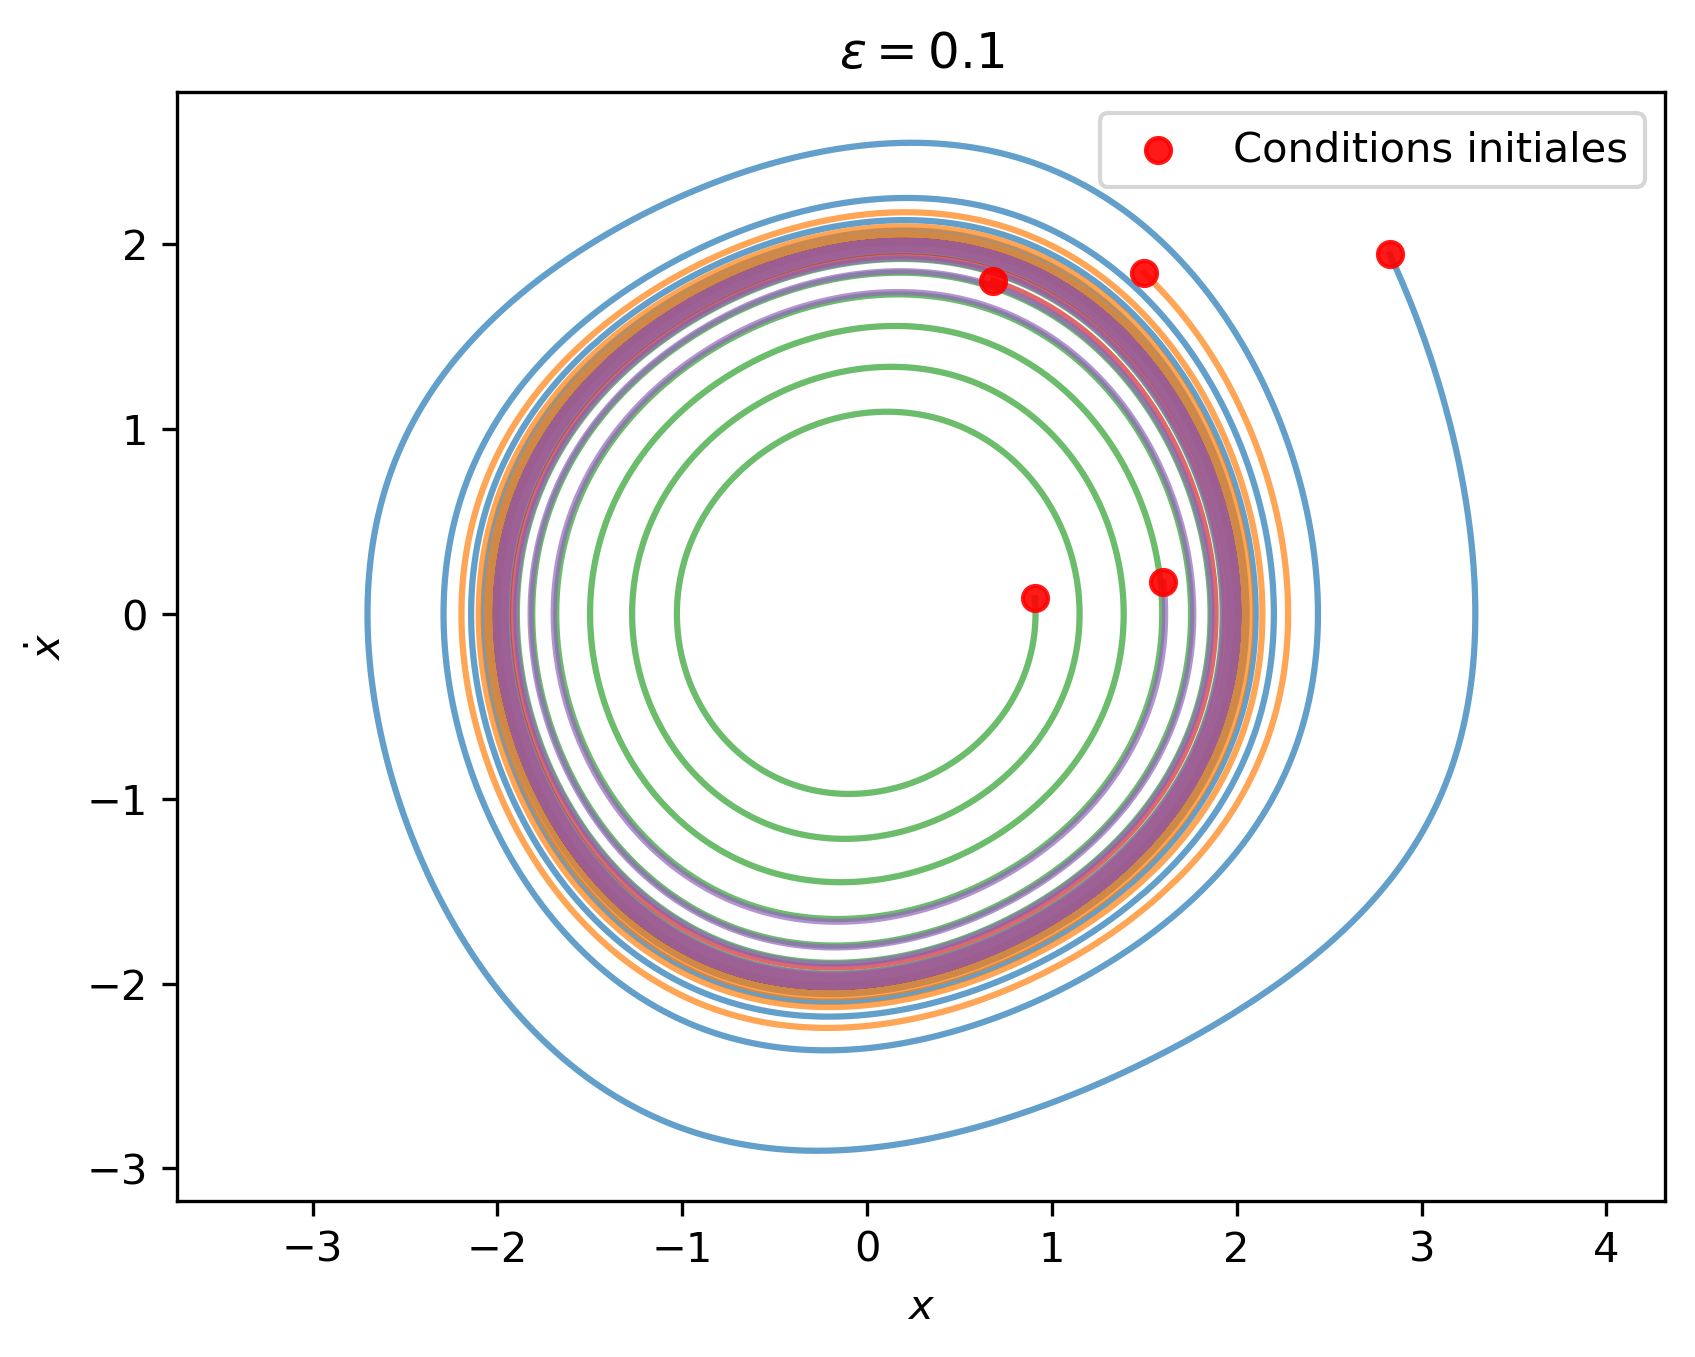
\includegraphics[width=0.45\textwidth]{images/vdp/vanderpol_small.png}
        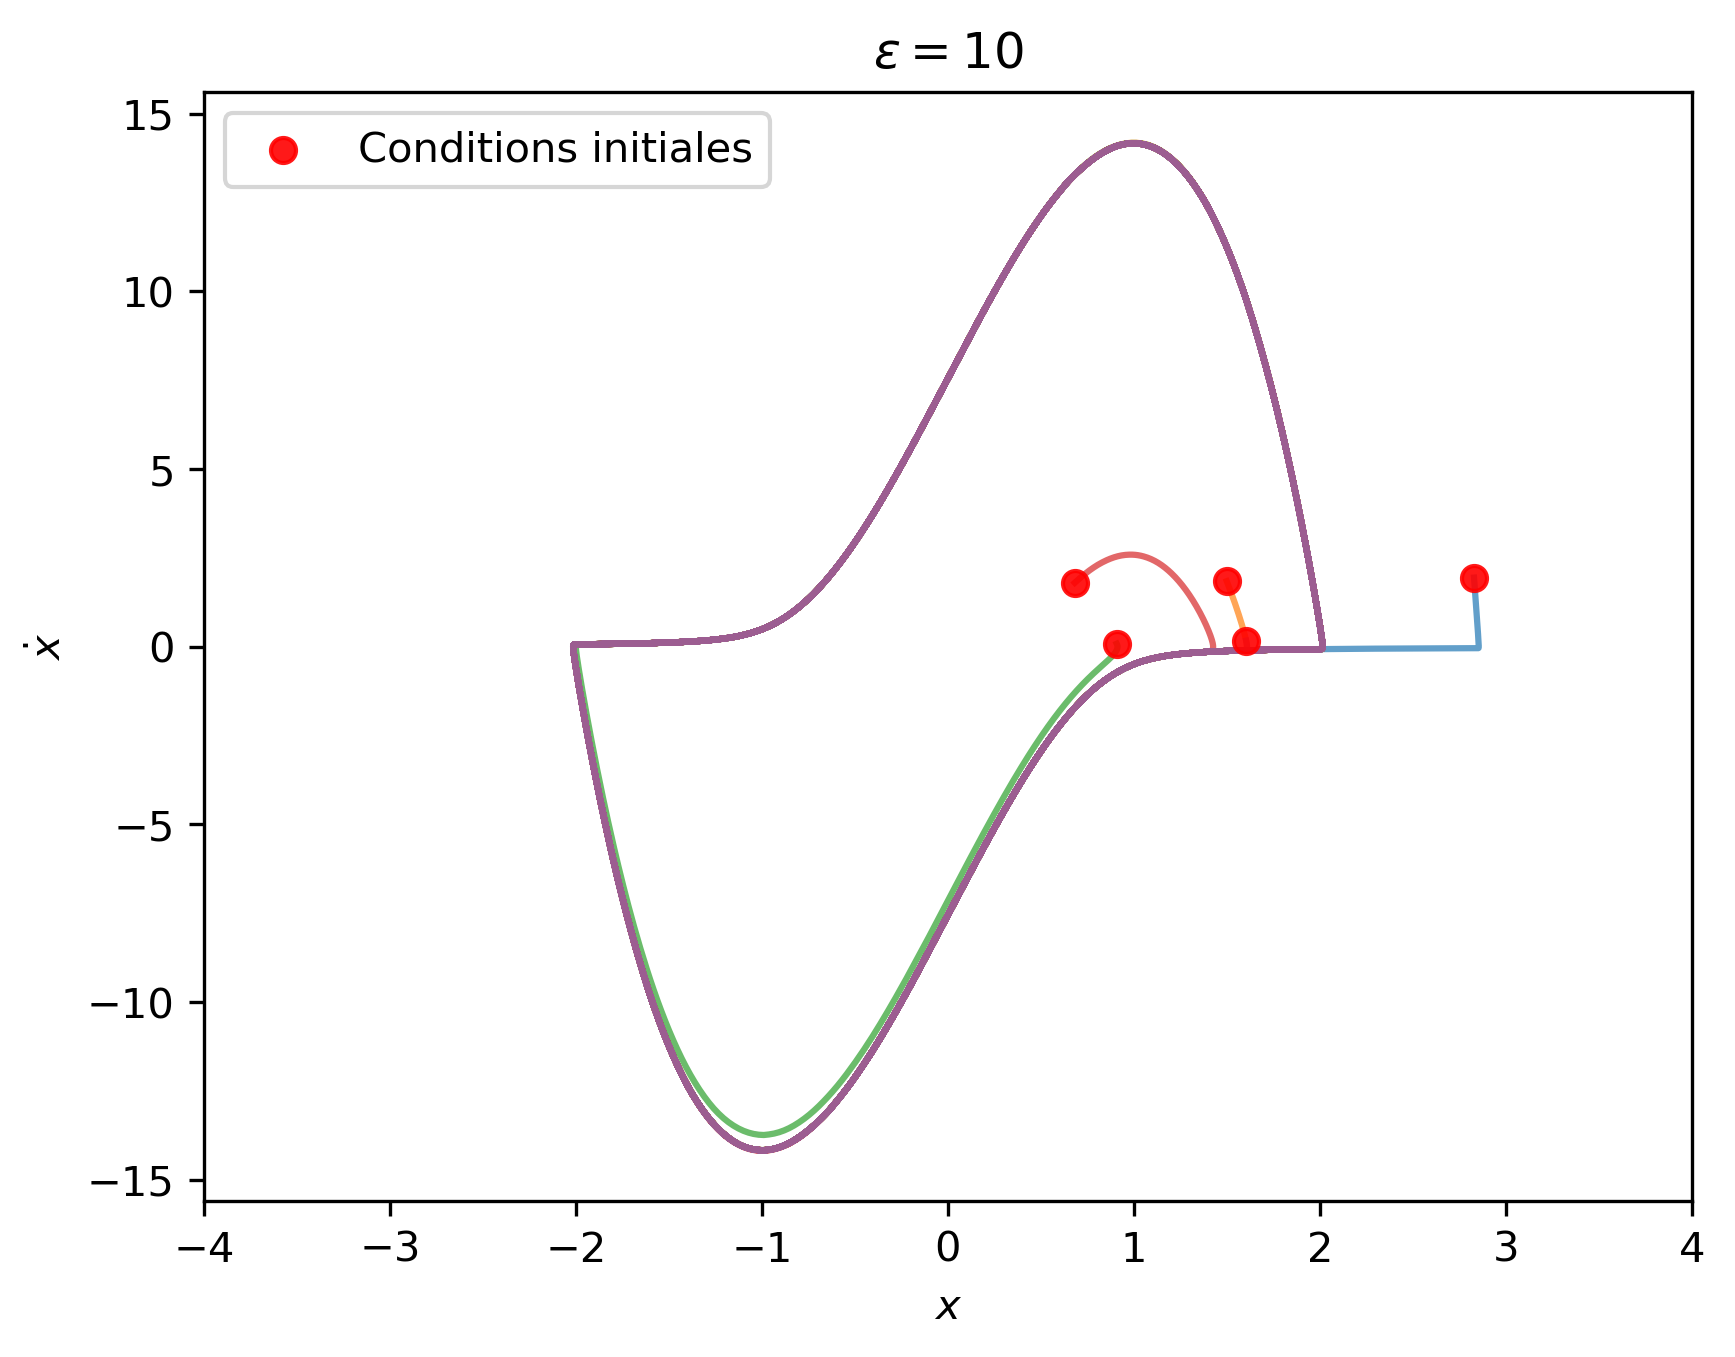
\includegraphics[width=0.45\textwidth]{images/vdp/vanderpol_large.png}
    \end{figure}

\end{frame}

\begin{frame}{Oscillateur de Van der Pol - 2}
    \begin{itemize}
      \item On peut trouver la fréquence angulaire $\omega$ du régime permanent avec méthode de Linsted \cite{rand_lecture_2012} :
      \[ \omega = 1 - \frac{1}{16}\epsilon^2 + O(\epsilon^3) \]
      \item Équations de mouvement après moyennement au premier ordre
      \begin{equation*}
        \left\{
        \begin{array}{@{}l@{}}
            \dot{r} = \frac{\epsilon}{8}r(4-r^2) \\
            \\
            \dot{\phi} = 0
        \end{array}
        \right.\,
        \qquad 
        x(t) = r(t)\cos(t+\phi_0)
      \end{equation*}
    \item Pas de phase de référence, c.a.d que $\phi_0$ dépend purement des conditions initiales et non du système
    \end{itemize}
  \end{frame}

% Section 3: Synchronization
% \section{Synchronisation}
% \begin{frame}{Que est-ce la synchronisation ?}
%   \begin{itemize}
%     \item Definition of synchronization {phase and amplitude}
%     \item Importance in various fields
%   \end{itemize}
% \end{frame}

% Section 3: Synchronization
\section{Synchronisation}
\begin{frame}{Que est-ce la synchronisation ?}
  \begin{itemize}
    \item Phénomène où plusieurs oscillateurs verouille leurs phase l'un par rapport à l'autre \cite{matheny_phase_2014}
    \item \emph{Phase locking}
  \end{itemize}
\end{frame}

\begin{frame}{Oscillateurs à cycle limite couplés}
  \begin{itemize}
    \item Système de deux oscillateurs de Van der Pol couplée
    \begin{equation*}
      \left\{\begin{array}{@{}l@{}}
      \ddot{x}_1 + x_1  + \epsilon(x_1^2 - 1)\dot{x}_1 = \epsilon k(x_2 - x_1) \\
      \\
      \ddot{x}_2 + x_2 + \epsilon(x_2^2 - 1)\dot{x}_2 = \epsilon k(x_1 - x_2)
    \end{array}\right.\, 
    \end{equation*}
    \item Après moyennement, $\Theta = \phi_2 - \phi_1$
    \tiny
    \begin{equation*}
      \left\{\begin{array}{@{}l@{}}
        \dot{r}_1 =  \frac{\epsilon}{8} r_1 \left( 4 - r_2^2 \right) + \epsilon k\frac{r_2}{2}\sin(\phi_2 - \phi_1)\\
        \\
        \dot{r}_2 =  \frac{\epsilon}{8} r_2 \left( 4 - r_2^2 \right) + \epsilon k\frac{r_1}{2}\sin(\phi_1 - \phi_2)\\
        \\
        \dot{\phi}_1 = \epsilon \frac{k}{2}\left( 1 - \frac{r_2}{r_1}\cos(\phi_2 - \phi_1)\right) \\
        \\
        \dot{\phi}_2 = \epsilon \frac{k}{2}\left( 1 - \frac{r_1}{r_2}\cos(\phi_1 - \phi_2)\right)
    \end{array}\right.\,
    \implies
      \left\{\begin{array}{@{}l@{}}
        \dot{r}_1 = \frac{\epsilon}{8} r_1 \left( 4 - r_2^2 \right) + \epsilon k\frac{r_2}{2}\sin(\Theta)\\
        \\
        \dot{r}_2 = \frac{\epsilon}{8} r_2 \left( 4 - r_2^2 \right) - \epsilon k\frac{r_1}{2}\sin(\Theta) \\
        \\
      \dot{\Theta} = \epsilon \frac{k}{2}\left(  \frac{r_2}{r_1} - \frac{r_1}{r_2} \right)\cos(\Theta)
    \end{array}\right.\,
    \end{equation*}
    \small
    \item On peut vérifier l'existence des solutions stationnaires $r_1=r_2=2$ avec $\Theta=0$ ou $\Theta=\pi$
  \end{itemize}
\end{frame}
    %     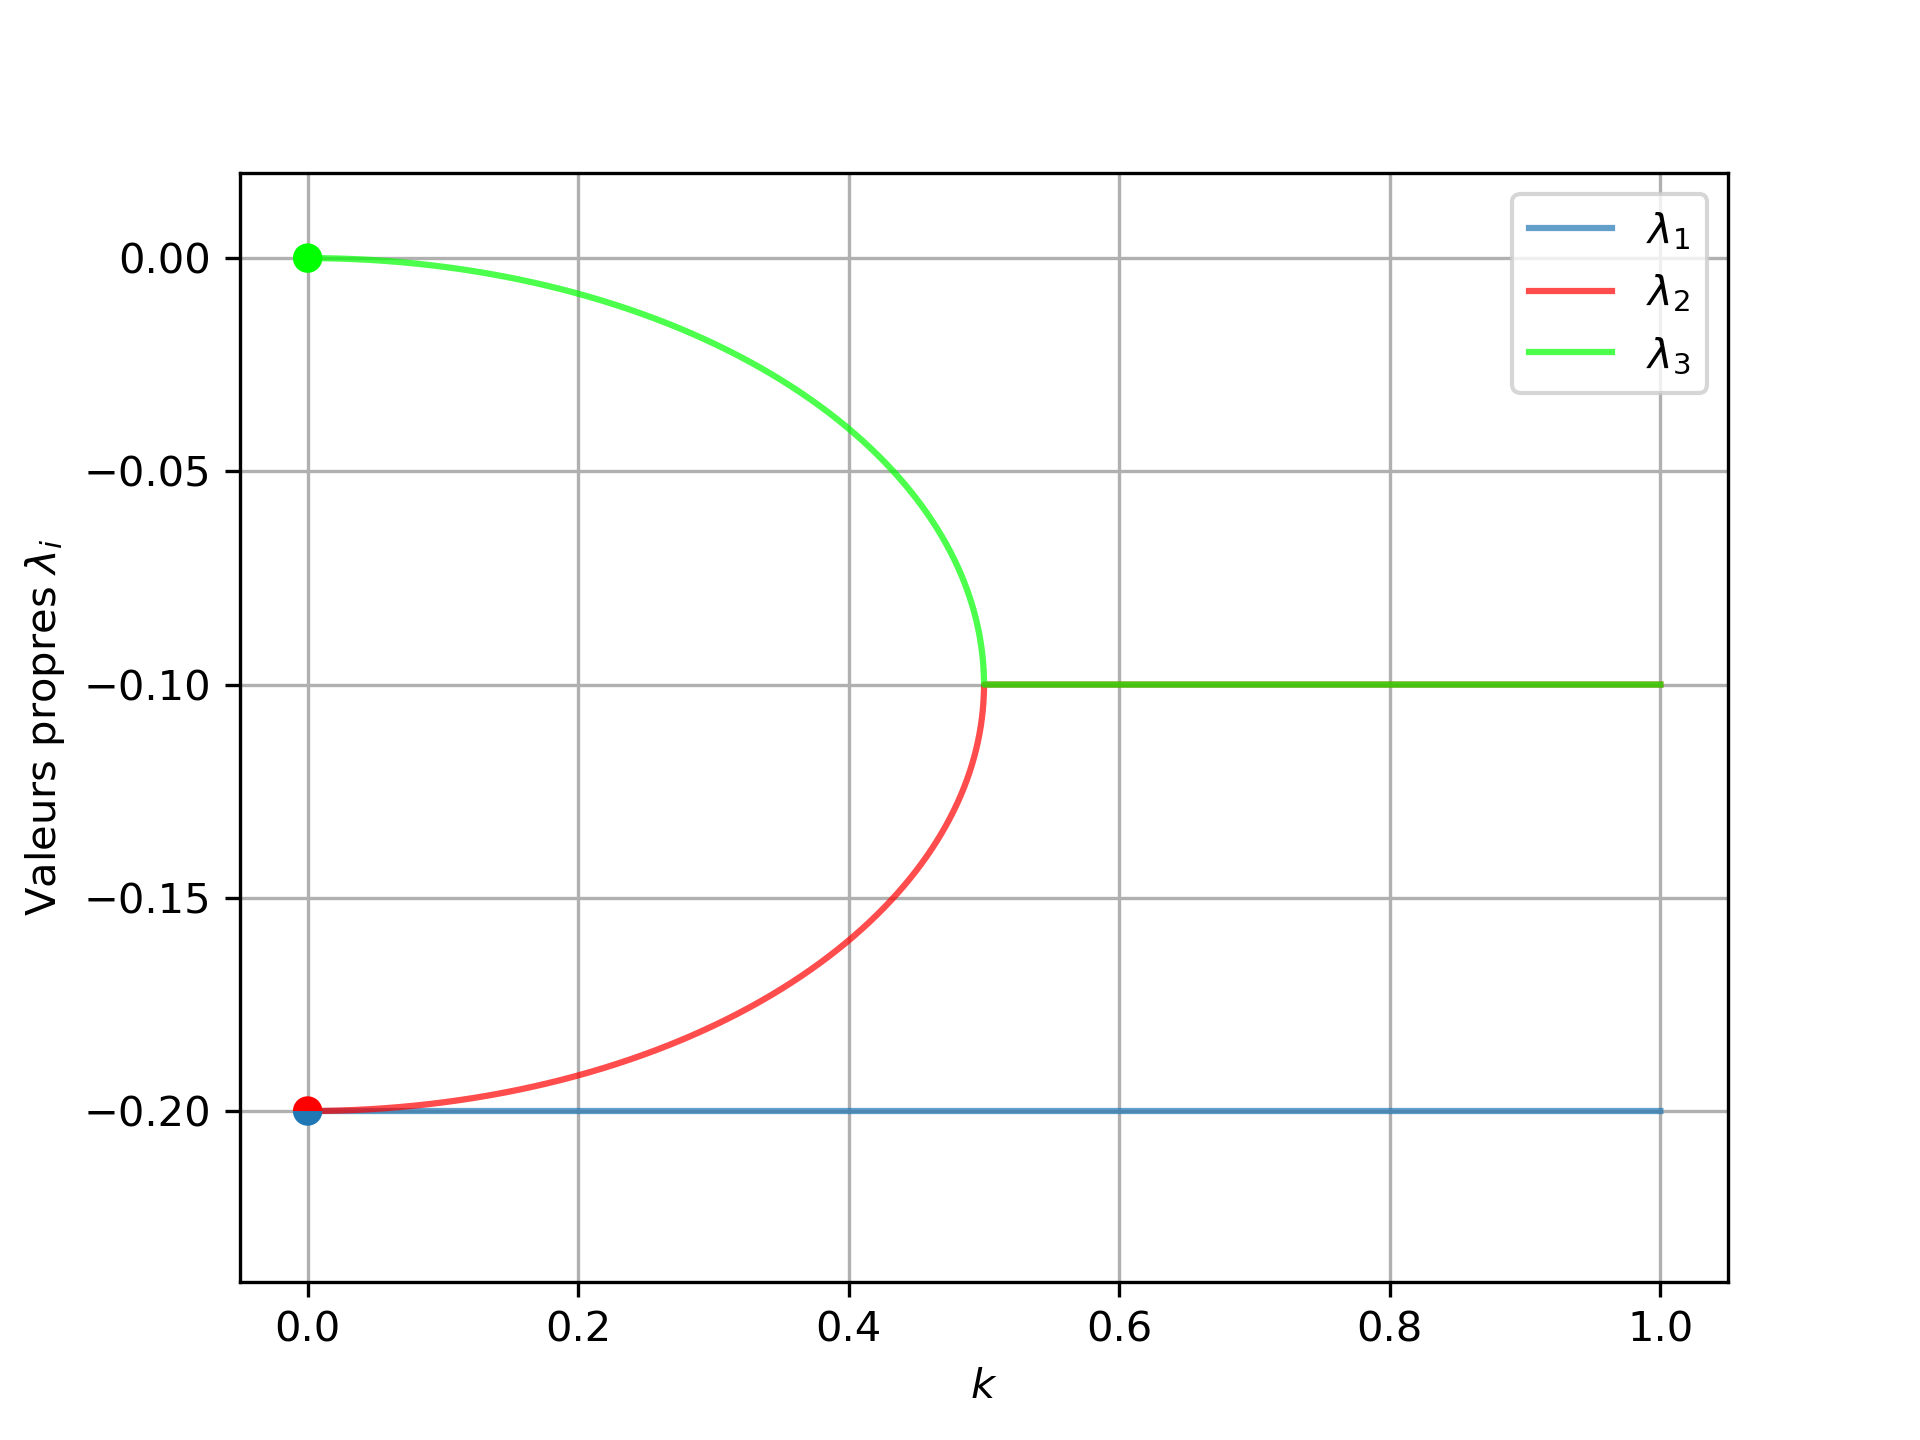
\includegraphics[width=\linewidth]{images/couplee/eigenvalues_eps=0.2.png}%

\begin{frame}{Oscillateurs à cycle limite couplés - 2}
  \begin{itemize}
    \item L'analyse de stabilité linéaire montre que ce sont des solutions stationnaires stable (valeurs propres négatives)
      \item La dynamique autour des deux points sont identiques
  \end{itemize}
  \begin{figure}
    \centering
    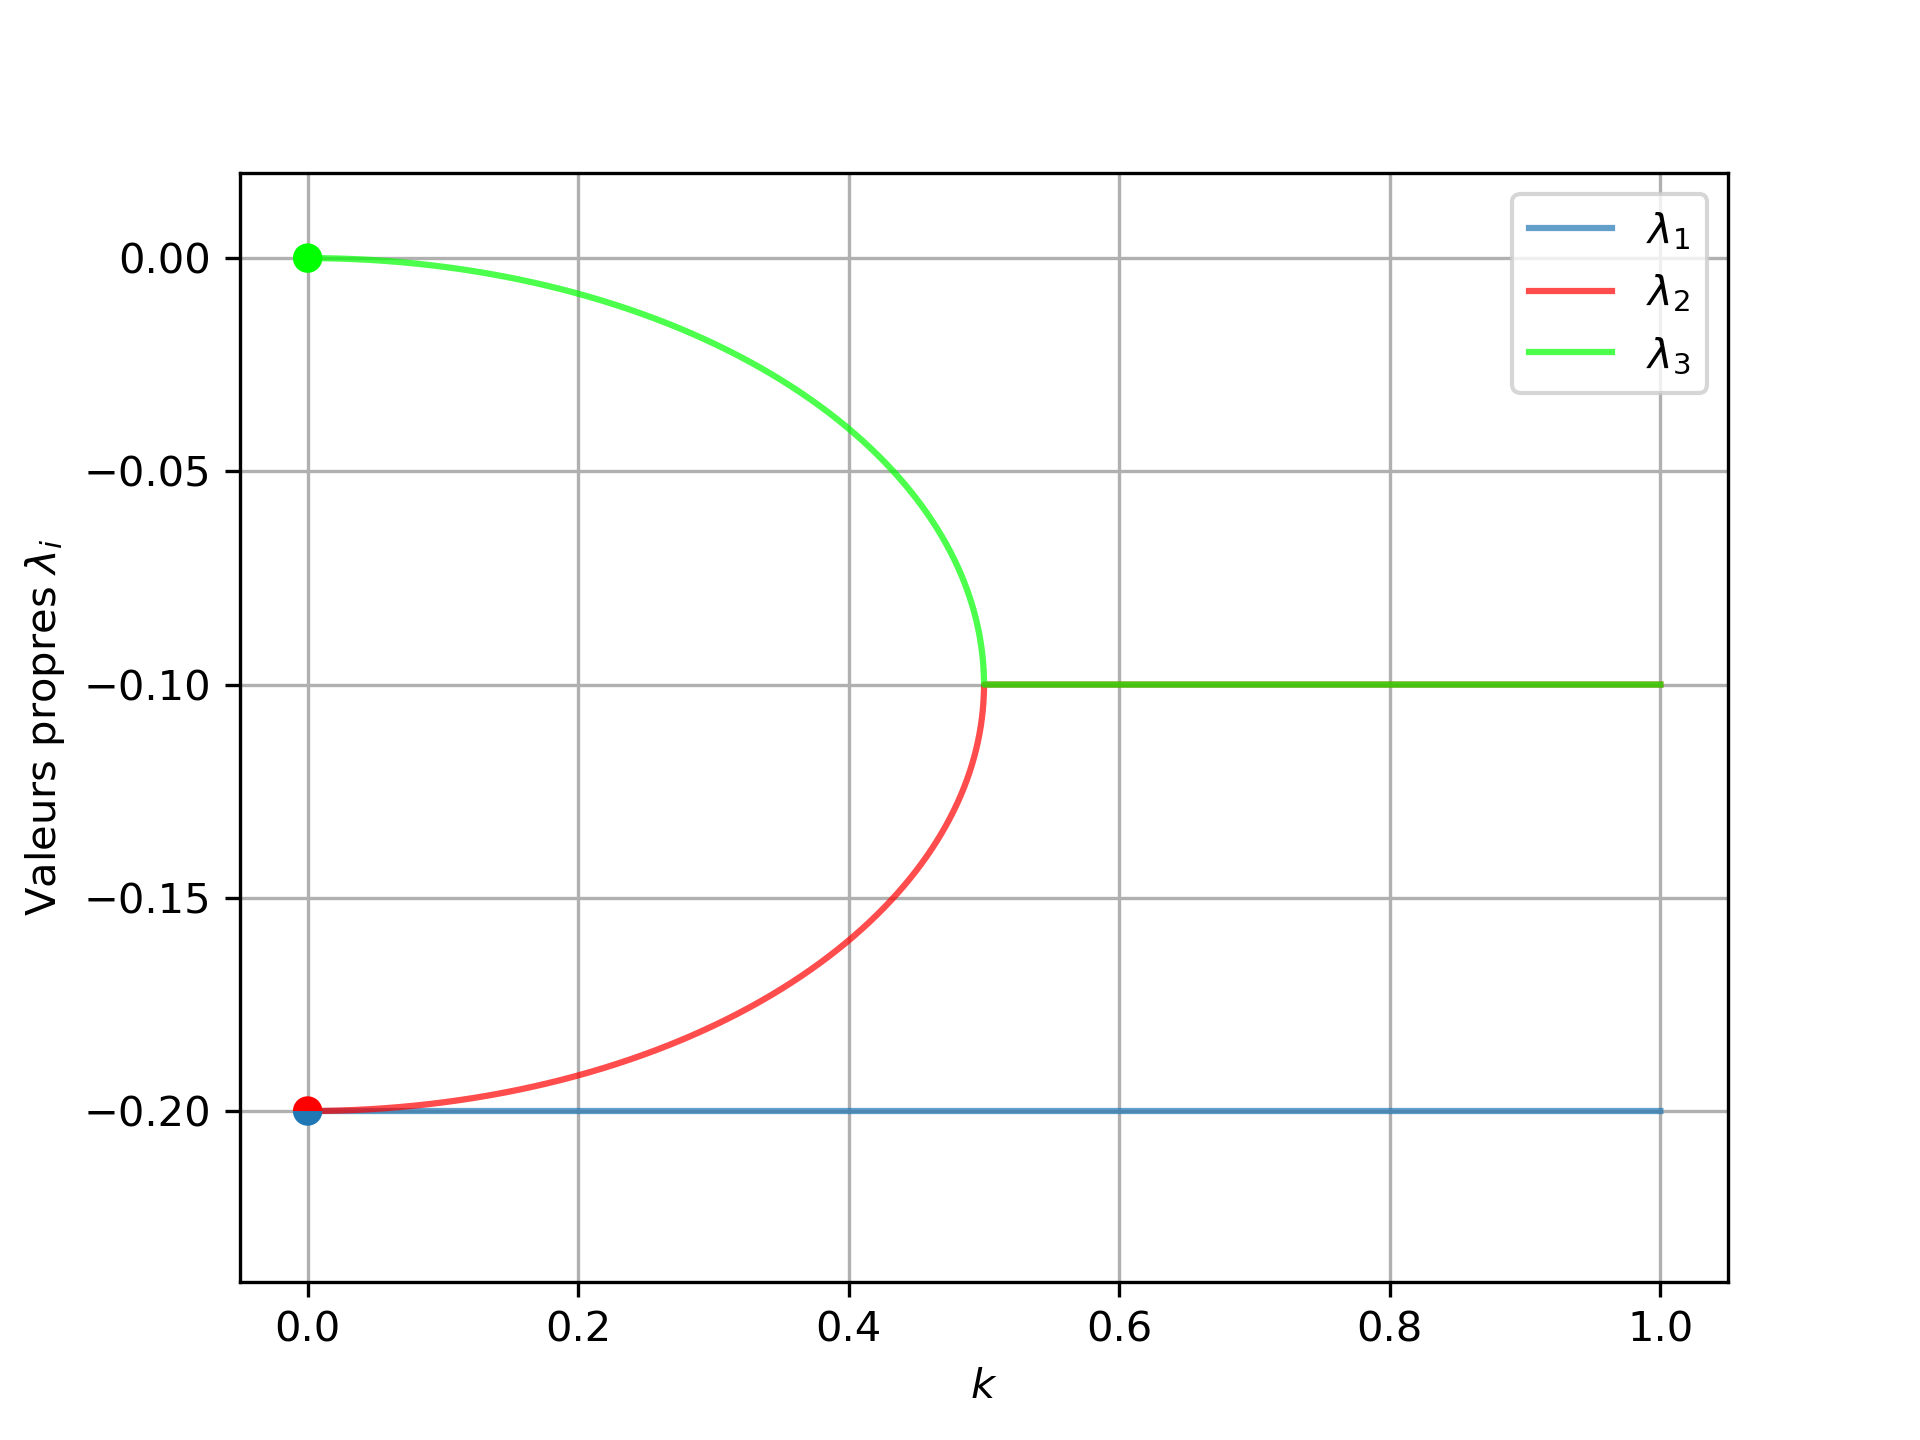
\includegraphics[width=0.37\textwidth]{images/couplee/eigenvalues_eps=0.2.png}
    \hfill
    \includegraphics[width=0.62\textwidth]{images/couplee/llabel_k=1_x0=[0.038,-0.018,0.265,-0.486]_ϵ=0.1.png}
\end{figure}
\end{frame}

% % Section 4: Applications
% \section{Applications}
% \begin{frame}{Applications of Non-Linear Oscillators and Synchronization}
%   \begin{itemize}
%     \item Nanotechnologies
%     \item Communication systems
%     \item Biological systems
%   \end{itemize}
% \end{frame}

% Section 5: Conclusion
\section{Conclusion}
\begin{frame}{Conclusion et autres perspectives}
  \begin{itemize}
    \item Oscillateurs non-identiques
    \item Réseau d'oscillateurs
    \item Modéliser systèmes réelles
  \end{itemize}
\end{frame}

\begin{frame}[allowframebreaks, noframenumbering]{Bibliographie}
    \TINY
    \printbibliography
\end{frame}

%\printbibliography

\end{document}
